% oss-plantilla: oss-2026.11
% Preámbulo corporativo fijo. No editar en sd-NN.tex: exportar_latex.py verificar lo compara byte a byte.
% Para cambiar el formato, editar esta plantilla u oss.sty y subir la versión de la primera línea.
\PassOptionsToPackage{unicode}{hyperref}
\PassOptionsToPackage{hyphens}{url}
\documentclass[11pt]{article}
\usepackage{amsmath,amssymb}
\usepackage{iftex}
\ifPDFTeX
  % Prism y otros editores en la nube: pdfLaTeX con Helvetica como familia por defecto.
  \usepackage[T1]{fontenc}
  \usepackage[utf8]{inputenc}
  \usepackage{textcomp}
  \usepackage[scaled=0.92]{helvet}
  \renewcommand{\familydefault}{\sfdefault}
  \DeclareUnicodeCharacter{2264}{\ensuremath{\leq}}
  \DeclareUnicodeCharacter{2265}{\ensuremath{\geq}}
  \DeclareUnicodeCharacter{2260}{\ensuremath{\neq}}
  \DeclareUnicodeCharacter{2248}{\ensuremath{\approx}}
  \DeclareUnicodeCharacter{2190}{\ensuremath{\leftarrow}}
  \DeclareUnicodeCharacter{2192}{\ensuremath{\rightarrow}}
  \DeclareUnicodeCharacter{25CF}{\ensuremath{\bullet}}
  \DeclareUnicodeCharacter{2713}{\ensuremath{\checkmark}}
\else
  % XeLaTeX/LuaLaTeX (compilación oficial local): DejaVu Sans.
  \usepackage{fontspec}
  \defaultfontfeatures{Ligatures=TeX,Scale=MatchLowercase}
  \setmainfont{DejaVu Sans}
  \setsansfont{DejaVu Sans}
  \setmonofont{DejaVu Sans Mono}
\fi
\usepackage[letterpaper,margin=20mm]{geometry}
\usepackage{microtype}
\usepackage{parskip}
\usepackage{xcolor}
\usepackage{longtable,booktabs,array}
\usepackage{calc}
\usepackage{etoolbox}
\makeatletter
\patchcmd\longtable{\par}{\if@noskipsec\mbox{}\fi\par}{}{}
\makeatother
\usepackage{footnotehyper}
\makesavenoteenv{longtable}
\usepackage{graphicx}
\makeatletter
\newsavebox\pandoc@box
\newcommand*\pandocbounded[1]{%
  \sbox\pandoc@box{#1}%
  \Gscale@div\@tempa{\textheight}{\dimexpr\ht\pandoc@box+\dp\pandoc@box\relax}%
  \Gscale@div\@tempb{\linewidth}{\wd\pandoc@box}%
  \ifdim\@tempb\p@<\@tempa\p@\let\@tempa\@tempb\fi
  \ifdim\@tempa\p@<\p@\scalebox{\@tempa}{\usebox\pandoc@box}%
  \else\usebox{\pandoc@box}%
  \fi}
\def\maxwidth{\ifdim\Gin@nat@width>\linewidth\linewidth\else\Gin@nat@width\fi}
\def\maxheight{\ifdim\Gin@nat@height>\textheight\textheight\else\Gin@nat@height\fi}
\makeatother
\setkeys{Gin}{width=\maxwidth,height=\maxheight,keepaspectratio}
\makeatletter
\def\fps@figure{htbp}
\makeatother
\usepackage[normalem]{ulem}
\providecommand{\st}[1]{\sout{#1}}
\usepackage{fancyvrb}
\setlength{\emergencystretch}{3em}
\providecommand{\tightlist}{%
  \setlength{\itemsep}{0pt}\setlength{\parskip}{0pt}}
\providecommand{\passthrough}[1]{#1}
\setcounter{secnumdepth}{-\maxdimen}
\ifPDFTeX
  \usepackage[spanish]{babel}
\else
  \usepackage[bidi=default]{babel}
  \babelprovide[main,import]{spanish}
\fi
\let\LanguageShortHands\languageshorthands
\def\languageshorthands#1{}
\usepackage{bookmark}
\usepackage{xurl}
\urlstyle{same}
\hypersetup{pdflang={es-CL},pdfcreator={Only Simple Solutions - exportar_latex.py}}
\usepackage{oss}
\begin{document}
\makeatletter
\newcommand{\ossFigCaption}[1]{\def\@captype{figure}\caption{#1}}
\makeatother
\renewcommand{\tablename}{Tabla}
\renewcommand{\figurename}{Figura}
\renewcommand{\thefigure}{7.\arabic{figure}}
\renewcommand{\thetable}{7.\arabic{table}}

\ossCover{Plan de trabajo, EDT, cronograma e implantación}{Subdocumento 7}
\tableofcontents
\clearpage

\section{Capítulo 7 · Introducción al Plan de trabajo}\label{capuxedtulo-7-introducciuxf3n-al-plan-de-trabajo}

La Estructura de Descomposición del Trabajo (EDT) organiza lo que Only Simple Solutions debe entregar a Multitiendas Ancoa S.A. Esta permite reconocer qué trabajo incluye el proyecto y cómo se divide en partes que pueden asignarse, revisarse y aceptarse.

El apartado 7.1 descompone el 100 \% del alcance hasta entregables estimables y asignables, y resume el diccionario de esa estructura; el apartado 7.2 describe cómo se coordinan los equipos y cómo  se distribuye el esfuerzo; el apartado 7.3 presenta las fechas, las dependencias y las condiciones para poner la solución en funcionamiento dentro de los 56 meses del contrato; el Formulario T-14 reúne el detalle de las cuentas de control, con sus entregables, esfuerzos y criterios de aceptación; el Formulario T-15 detalla la distribución mensual de las horas hombre planificadas y la carga de trabajo por etapa y durante la operación; y el Formulario T-18 desarrolla la estrategia de implantación, las condiciones de liberación, los criterios de aceptación y los procedimientos de retorno ante fallas.

\section{7.1 EDT}\label{edt}

La Estructura de Descomposición del Trabajo (EDT) organiza el alcance del proyecto en entregables y paquetes de trabajo que permiten estimar el esfuerzo y asignar responsables. Su propósito es identificar qué debe completarse para entregar la solución, desde las actividades iniciales hasta el término de la operación.
La EDT comprende quince ramas que abarcan la gestión, el desarrollo y las integraciones, junto con la infraestructura, la seguridad, la calidad, la migración, las cinco innovaciones y la puesta en marcha. También incorpora la capacitación, la documentación y los servicios necesarios para sostener la solución durante el contrato. Estas ramas agrupan trabajos relacionados y pueden ejecutarse de forma simultánea; su numeración no representa una secuencia temporal.
En este apartado se presenta la estructura general y se explica el propósito de cada rama. El Formulario T-14 contiene el diccionario detallado, con los entregables, los criterios de aceptación, los responsables y el esfuerzo asignado. La secuencia de ejecución y su distribución en el tiempo se desarrollan en los apartados 7.2 y 7.3.

\subsection{7.1.1 Criterios de descomposición}

La EDT agrupa el trabajo por entregables, es decir, por resultados que el cliente puede revisar y validar durante el proyecto. Se aplica la regla del 100 \% para incluir todo el alcance comprometido, también el trabajo de seguridad, capacitación y soporte, conforme a la metodología del Capítulo 6.

La raíz 1.0 representa la solución completa y se divide en quince ramas. Cada rama reúne cuentas de control que agrupan entregables con un responsable y un esfuerzo estimable. Las cuentas se descomponen en paquetes de trabajo cuando se requiere mayor detalle. En el desarrollo de software, estos paquetes corresponden a casos de uso, entendidos como tareas que una persona realiza con el sistema para obtener un resultado.

Los códigos permiten seguir la relación entre cada parte y el conjunto. El formato 1.N identifica una rama; 1.N.M identifica una cuenta; y 1.N.M.S identifica un paquete de trabajo. Los nombres indican qué se entrega, mientras que el diccionario del T-14 especifica las condiciones que debe cumplir. Esta separación permite leer la estructura sin repetir en cada nombre todas las pruebas, cantidades y requisitos.

La estructura incluye las dos etapas de implementación y los 36 meses de operación. También incluye las cinco innovaciones del Subdocumento 13, desglosadas en 40 paquetes con estimación y ventanas explícitas en el anexo del T-14. Las ramas transversales, como dirección, seguridad y documentación, acompañan las etapas en que sus entregables son necesarios. La EDT cubre el trabajo posterior a la adjudicación; la preparación de la oferta queda fuera de su alcance.

\subsection{7.1.2 Estructura de la EDT}

La Figura 7.1 presenta la estructura general, desde la solución completa hasta sus quince ramas, mientras que la Tabla 7.1 resume el número de cuentas, el entregable principal y el responsable de cada rama, permitiendo ubicar tanto la construcción de la solución como el trabajo necesario para ponerla en servicio y mantenerla.

Las ramas agrupan tipos de entregables y pueden desarrollarse al mismo tiempo. Su numeración es solamente para identificarlas; el orden de ejecución y sus dependencias se explican en los apartados 7.2 y 7.3.

\begin{center}
\begin{minipage}{\linewidth}
\centering
\ossFigCaption{Estructura de descomposición del trabajo, con la raíz y las quince ramas.}\label{fig:7-1}
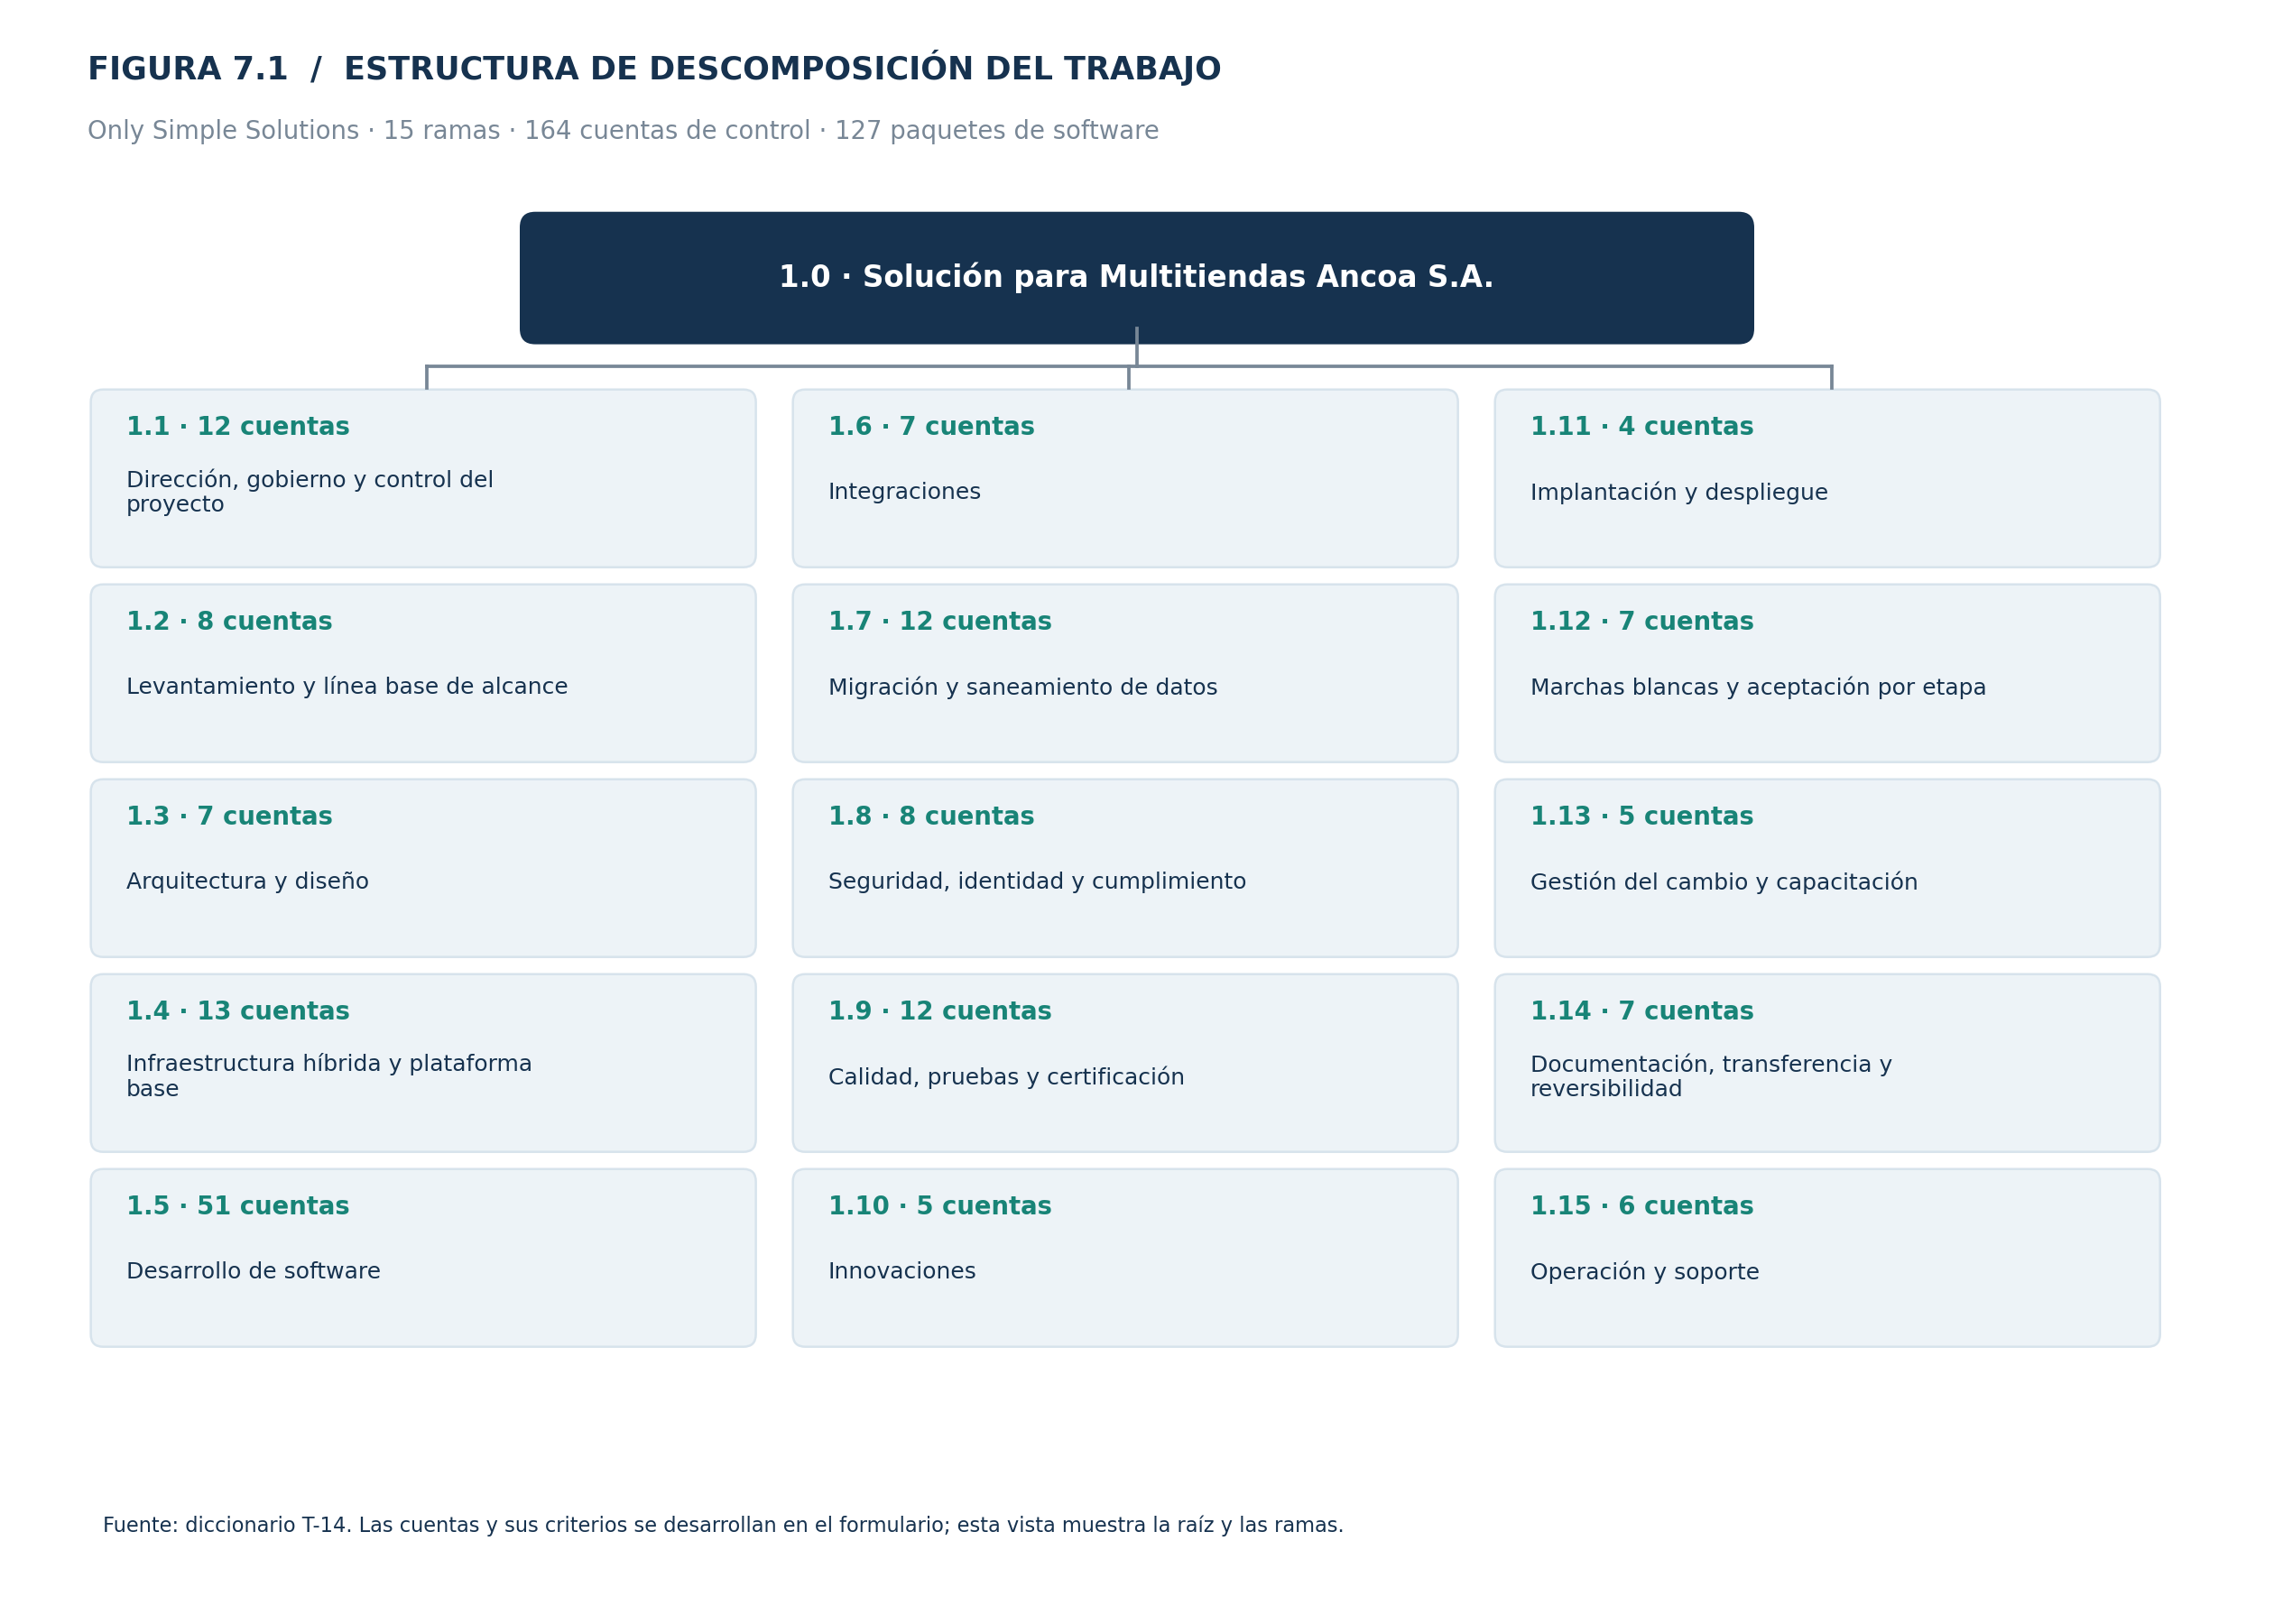
\includegraphics[width=\linewidth,height=\textheight,keepaspectratio]{figuras/sd07-figuras/sd07-edt1.0.png}
\raggedright\textbf{Fuente:} Elaboración propia.
\end{minipage}
\end{center}

La figura muestra la raíz y las quince ramas, con el número de cuentas de cada una. La Tabla 7.1 facilita la comparación entre ramas.

\begin{longtable}{p{0.24\linewidth}p{0.07\linewidth}p{0.2\linewidth}p{0.25\linewidth}p{0.12\linewidth}}
\caption{Diccionario resumido de la EDT por rama.}\label{tab:7-1}\\
\toprule\noalign{}
\textbf{Rama} & \textbf{Cuentas de control} & \textbf{Entregable principal} & \textbf{Criterio de aceptación (resumen)} & \textbf{Responsable} \\
\midrule
\endhead
\bottomrule
\multicolumn{5}{@{}l}{\rule{0pt}{3.2ex}\textbf{Fuente:} Elaboración propia.} \\
\endlastfoot
1.1 Dirección, gobierno y control del proyecto & 12 & Plan de dirección integrado & Aprobado por el comité del proyecto y actualizado en cada hito. & Jefe de Proyecto \\
1.2 Levantamiento y línea base de alcance & 8 & Línea base de alcance & Aprobada por el CLIENTE con el mapa de interfaces y la matriz de trazabilidad. & Líder Funcional \\
1.3 Arquitectura y diseño & 7 & Documento de arquitectura y catálogo de decisiones & Aprobado por el CLIENTE con la frontera Retail–Emisor segregada en el modelo de datos. & Arquitecto de Solución \\
1.4 Infraestructura híbrida y plataforma base & 13 & Infraestructura híbrida con ambientes habilitados & Ambientes de Desarrollo, Calidad, Preproducción, Producción y Recuperación ante desastres operativos con observabilidad. & Arquitecto de Solución \\
1.5 Desarrollo de software & 51 (127 paquetes) & Software de cada servicio por etapa & Entregable por etapa con calidad aprobada y evidencia de cobertura. & Líder de Desarrollo \\
1.6 Integraciones & 7 & Catálogo de interfaces y contratos & Interfaces certificadas sin diferencias con el mapa AS-IS aprobado. & Líder de Integración \\
1.7 Migración y saneamiento de datos & 12 & Datos saneados, migrados y conciliados & Conciliación aprobada por acta y plataformas heredadas retiradas conforme al plan. & Líder de Datos \\
1.8 Seguridad, identidad y cumplimiento & 8 & Plan de seguridad y matriz de controles & Controles implementados y probados, con la remediación cerrada. & Encargado de Seguridad de la Información \\
1.9 Calidad, pruebas y certificación & 12 & Certificación de cada etapa & Pruebas de aceptación, carga, resiliencia y seguridad ofensiva aprobadas. & Líder de Calidad y Pruebas \\
1.10 Innovaciones & 5 & Las cinco innovaciones entregadas & Cada innovación aceptada con trazabilidad a arquitectura, EDT y flujo de caja. & Arquitecto de Solución \\
1.11 Implantación y despliegue & 4 & Plan de implantación y pipeline de despliegue & Despliegue y reversión probados antes de cada paso a producción. & Líder de Implantación y Gestión del Cambio \\
1.12 Resultados de las marchas blancas y aceptación por etapa & 7 & Actas de aceptación de la Etapa 1 y de la Etapa 2 & Marcha blanca cerrada conforme a sus indicadores en cada etapa. & Líder de Implantación y Gestión del Cambio \\
1.13 Gestión del cambio y capacitación & 5 & Personal capacitado y certificado & Asistencia y evaluación aprobadas en las jornadas de capacitación. & Líder de Implantación y Gestión del Cambio \\
1.14 Documentación, transferencia y reversibilidad & 7 & Documentación técnica y plan de reversibilidad & Entregados y aprobados antes del cierre contractual. & Jefe de Proyecto \\
1.15 Operación y soporte & 6 & Operación con niveles de servicio cumplidos & Informes de nivel de servicio aceptados y recuperación probada semestralmente. & Líder de Operación / SRE \\
\end{longtable}


Las quince ramas suman 164 cuentas de control. La rama 1.5 concentra 127 paquetes de software, mientras que las demás reúnen los entregables de preparación, control, implantación y operación. El Formulario T-14 desarrolla el detalle que corresponde a cada cuenta; los párrafos siguientes explican para qué sirve cada rama dentro del proyecto.

\subsection{7.1.3 Descripción de las ramas de la EDT}

Cada rama responde a una necesidad concreta de la solución, y su descripción permite entender qué resultado se espera y cómo se relaciona con el trabajo de las otras ramas. Las condiciones precisas de aceptación se consultan en las cuentas del mismo código en el Formulario T-14.

\subsubsection{7.1.3.1 Dirección, gobierno y control del proyecto (EDT 1.1)}

Esta rama organiza la conducción del proyecto y la relación de trabajo entre Only Simple Solutions y Ancoa. Su objetivo es que las decisiones, los compromisos y los cambios puedan seguirse durante todo el contrato. El plan de dirección establece cómo se coordina el equipo y cómo se revisa el avance. Las actas de los comités dejan constancia de los acuerdos y permiten identificar qué debe resolver cada responsable antes de la siguiente revisión.

La Figura 7.2 presenta las 12 cuentas de control de esta rama, alineadas en un mismo nivel bajo el entregable principal.

\begin{center}
\begin{minipage}{\linewidth}
\centering
\ossFigCaption{EDT resumida de la rama 1.1}\label{fig:7-2}
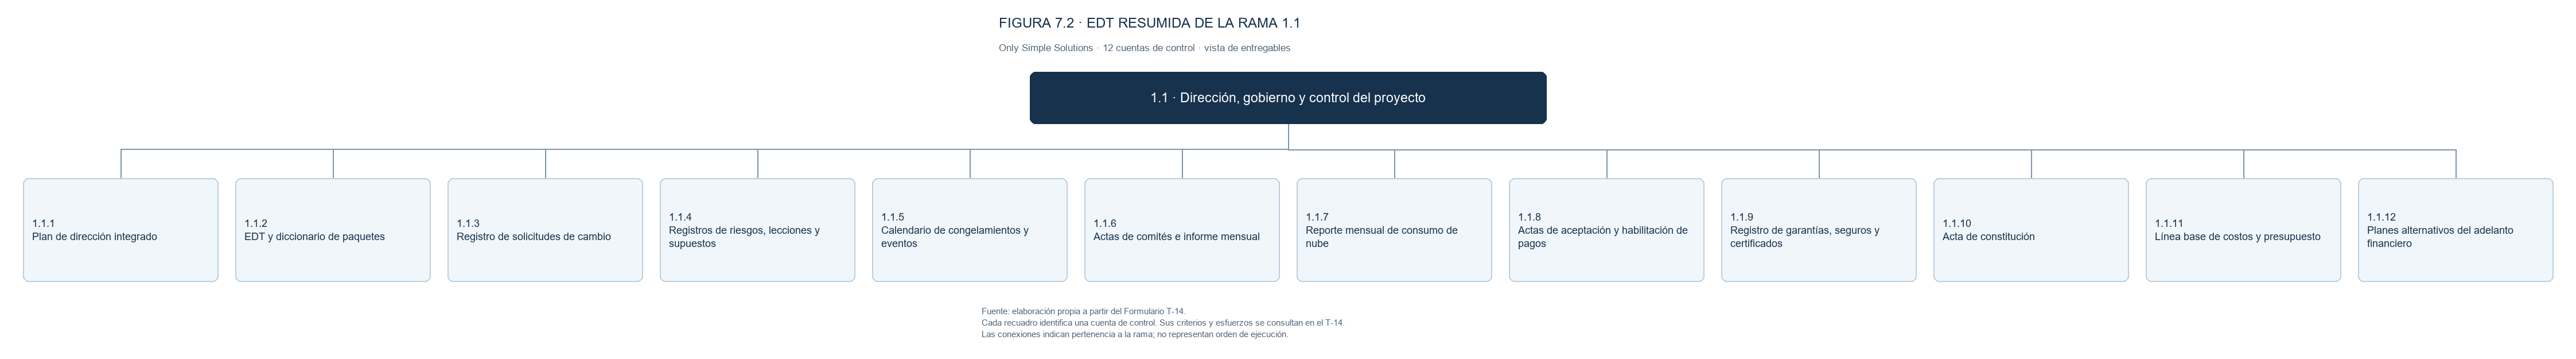
\includegraphics[width=\linewidth,height=\textheight,keepaspectratio]{figuras/sd07-figuras/sd07-edt1.1.png}
\raggedright\textbf{Fuente:} Elaboración propia a partir del Formulario T-14.
\end{minipage}
\end{center}

El trabajo comprende el seguimiento de riesgos, las solicitudes de cambio y los supuestos que todavía necesitan confirmación. Por ejemplo, si una modificación afecta un entregable, su evaluación debe indicar qué consecuencias tiene sobre el alcance, los recursos y el plazo antes de incorporarla al plan. También se mantiene el calendario de eventos y congelamientos, que identifica los períodos en que deben restringirse los cambios en los sistemas utilizados por el negocio.

Los resultados de esta rama son documentos de gestión vigentes y registros que permiten comprobar el estado del proyecto. Incluyen los informes de avance, las aceptaciones y el control de obligaciones contractuales. Esta información reúne antecedentes de las demás ramas y sirve para decidir acciones cuando aparecen desviaciones. El seguimiento continúa durante la operación, según la ventana de cada cuenta del T-14.

\subsubsection{7.1.3.2 Levantamiento y línea base de alcance (EDT 1.2)}

El levantamiento permite comprender cómo trabaja Ancoa antes de completar el diseño de la solución. Su propósito es acordar qué problemas debe resolver el proyecto, qué funciones se entregarán y qué condiciones deben cumplirse para aceptarlas. Para ello se documentan los procesos, las reglas del negocio y los volúmenes de información. También se revisa cómo se comunican las plataformas existentes, porque una modificación puede afectar a varios sistemas y áreas de la empresa.

La Figura 7.3 presenta las 8 cuentas de control de esta rama, alineadas en un mismo nivel bajo el entregable principal.

\begin{center}
\begin{minipage}{\linewidth}
\centering
\ossFigCaption{EDT resumida de la rama 1.2}\label{fig:7-3}
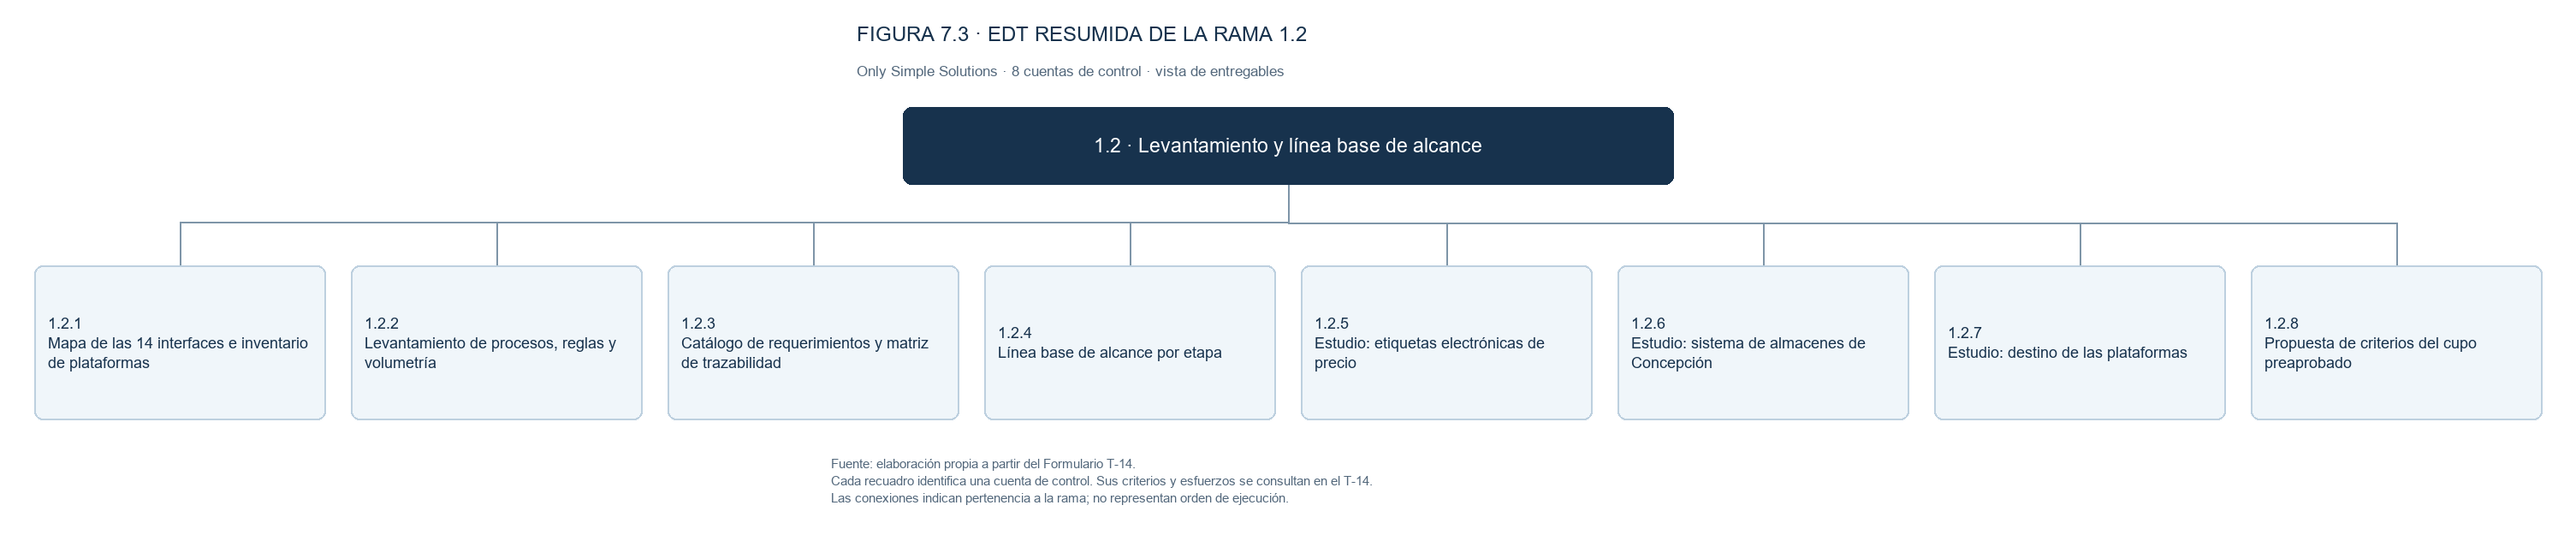
\includegraphics[width=\linewidth,height=\textheight,keepaspectratio]{figuras/sd07-figuras/sd07-edt1.2.png}
\raggedright\textbf{Fuente:} Elaboración propia a partir del Formulario T-14.
\end{minipage}
\end{center}

A partir de esos antecedentes se prepara la línea base de alcance, que corresponde a la versión aprobada de lo que incluye cada etapa. El catálogo de requerimientos y su matriz de trazabilidad permiten relacionar cada necesidad con el componente y el entregable que la atenderán. La rama también considera la evaluación de etiquetas electrónicas de precio, la incorporación del centro de distribución de Concepción a un sistema de gestión de almacenes y la definición del destino de las plataformas actuales (Multitiendas Ancoa S.A., 2026, Caso 09, cap. 5, p. 13; cap. 10, restricción 14, p. 26; cap. 11, p. 26). Las alternativas se fundamentan en la propuesta y se someten a la aprobación que corresponda.

El resultado esperado es un alcance entendido de la misma forma por el cliente y el equipo ejecutor. Sus definiciones alimentan la arquitectura, la construcción y las pruebas de aceptación. Cuando se inicia el trabajo de la segunda etapa, se actualiza su alcance conforme a las cuentas del T-14. Las exclusiones y los supuestos quedan documentados para evitar que una expectativa se confunda con un compromiso aprobado.

\subsubsection{7.1.3.3 Arquitectura y diseño (EDT 1.3)}

La arquitectura convierte las necesidades acordadas en una descripción de cómo funcionará la solución. Explica qué responsabilidad tiene cada componente, dónde se instalará y qué información podrá intercambiar. En Ancoa, esta definición debe respetar la separación entre la actividad comercial y el emisor de crédito (Multitiendas Ancoa S.A., 2026, Caso 09, cap. 13, núm. 13.3, condición 7, p. 30). Por ello, el diseño documenta los límites de sus datos y los intercambios autorizados, de manera que las funciones compartidas mantengan esa separación.

La Figura 7.4 presenta las 7 cuentas de control de esta rama, alineadas en un mismo nivel bajo el entregable principal.

\begin{center}
\begin{minipage}{\linewidth}
\centering
\ossFigCaption{EDT resumida de la rama 1.3}\label{fig:7-4}
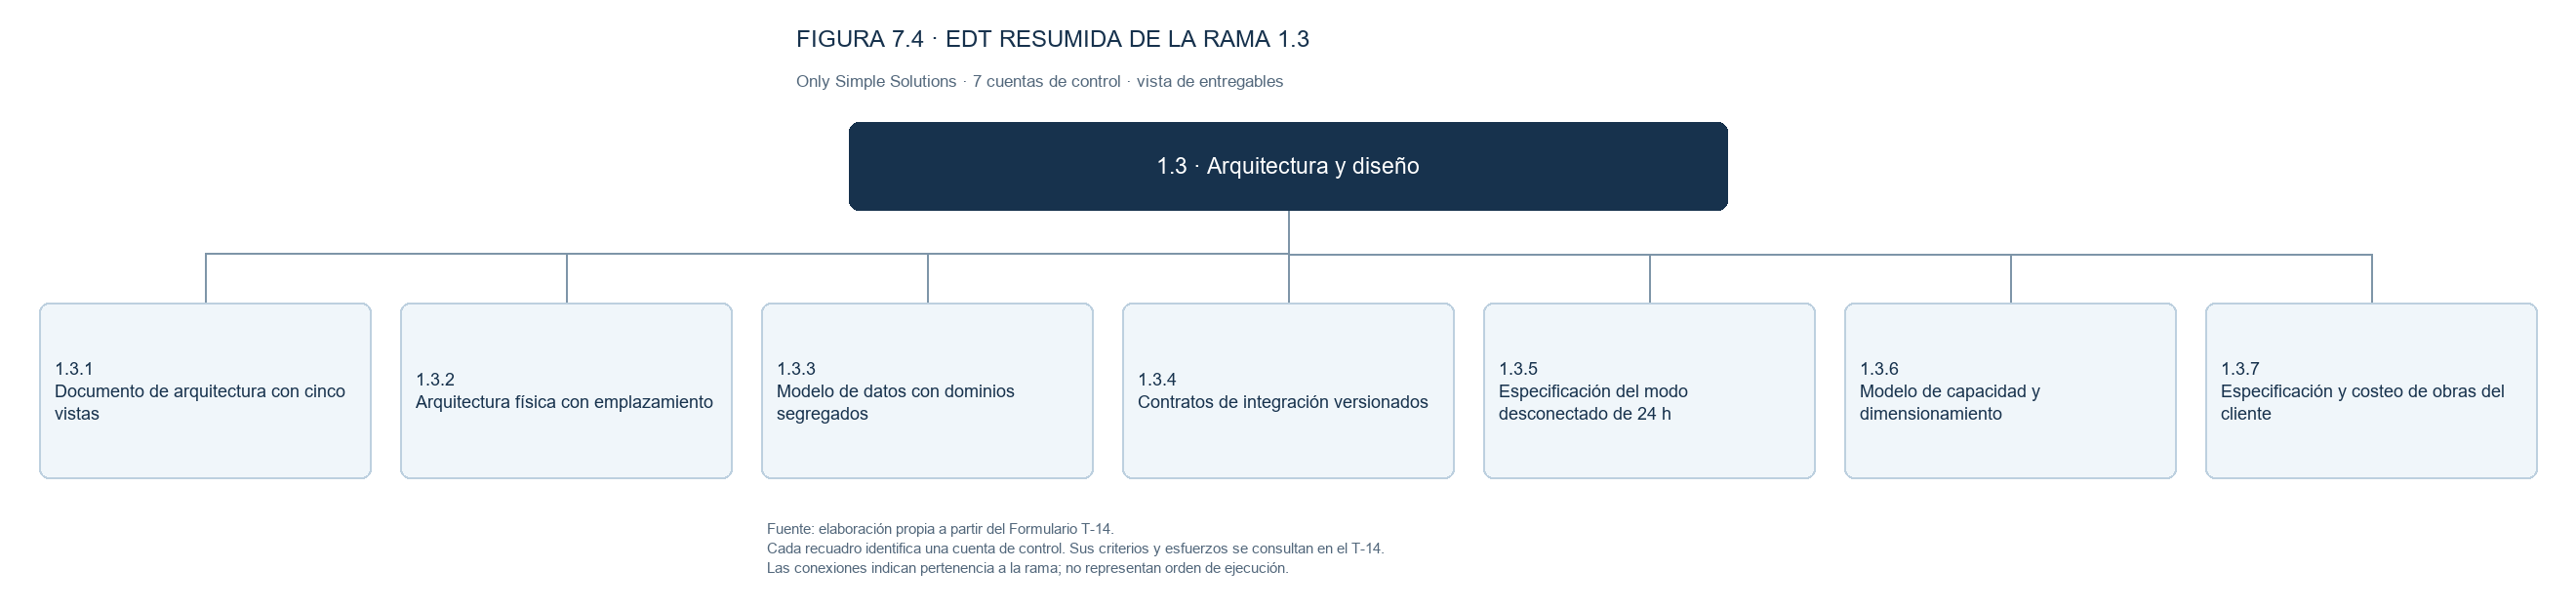
\includegraphics[width=\linewidth,height=\textheight,keepaspectratio]{figuras/sd07-figuras/sd07-edt1.3.png}
\raggedright\textbf{Fuente:} Elaboración propia a partir del Formulario T-14.
\end{minipage}
\end{center}

La rama reúne las vistas de la solución, el modelo de datos y las reglas de conexión entre sistemas. También define cómo operará una tienda cuando pierda el enlace y cómo se incorporarán sus operaciones al recuperar la comunicación. La continuidad de venta y cobro ante esa pérdida es una restricción del caso (Multitiendas Ancoa S.A., 2026, Caso 09, cap. 10, restricción 5, p. 26). El dimensionamiento estima la capacidad necesaria a partir de las cargas previstas. Las especificaciones físicas indican los requerimientos de instalación y las obras que debe ejecutar el cliente, según la distribución de responsabilidades establecida.

Estos documentos permiten que los equipos de infraestructura y desarrollo trabajen con criterios comunes. Las decisiones quedan registradas para comprender por qué se eligió una organización determinada y qué consecuencias tendría modificarla. La arquitectura entrega así una referencia para construir y comprobar la solución; la instalación efectiva de los medios tecnológicos y la programación de las funciones se desarrollan en las ramas 1.4 y 1.5.

\subsubsection{7.1.3.4 Infraestructura híbrida y plataforma base (EDT 1.4)}

Esta rama prepara los medios tecnológicos que necesita la solución para funcionar. La carga principal se sitúa en nube pública y se complementa con componentes en las dependencias de Ancoa. Esta distribución permite atender las necesidades centrales y las de los sitios que deben mantener funciones locales. El trabajo incluye configurar las redes y los entornos, con la separación requerida para el ámbito del emisor de crédito.

La Figura 7.5 presenta las 13 cuentas de control de esta rama, alineadas en un mismo nivel bajo el entregable principal.

\begin{center}
\begin{minipage}{\linewidth}
\centering
\ossFigCaption{EDT resumida de la rama 1.4}\label{fig:7-5}
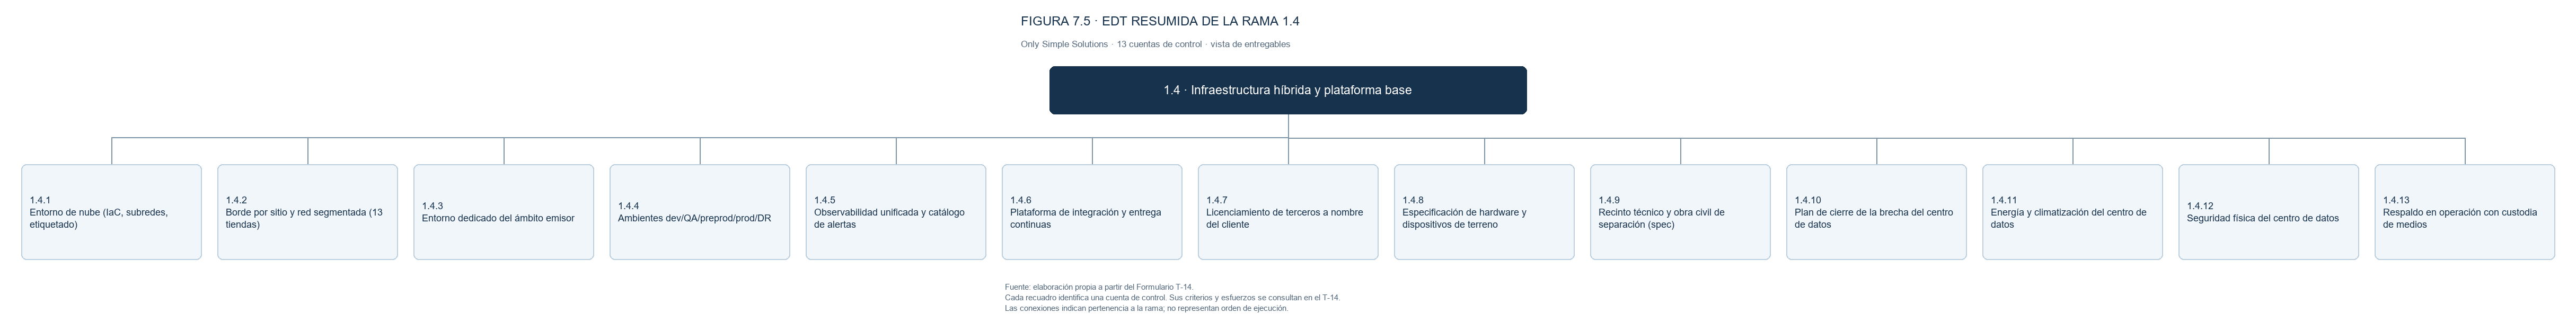
\includegraphics[width=\linewidth,height=\textheight,keepaspectratio]{figuras/sd07-figuras/sd07-edt1.4.png}
\raggedright\textbf{Fuente:} Elaboración propia a partir del Formulario T-14.
\end{minipage}
\end{center}


Se habilitan ambientes diferenciados para desarrollar, comprobar la calidad, ensayar antes de la puesta en servicio, operar y recuperar la solución ante desastres. Un ambiente es un espacio tecnológico preparado para un uso específico; separarlos permite realizar pruebas sin intervenir directamente sobre la operación real. La rama incorpora además respaldos, alertas y herramientas para instalar versiones de forma repetible. Las alertas permiten advertir condiciones que podrían afectar el servicio y los respaldos deben demostrar que la información puede recuperarse.

Las entregas parciales de infraestructura permiten iniciar ensayos antes de completar la plataforma integrada. También se preparan las especificaciones de equipos y de las condiciones físicas, como energía, climatización y control de acceso. El resultado de esta rama debe ser una plataforma configurada y comprobada, sobre la que puedan trabajar los equipos de software, pruebas y operación.

\subsubsection{7.1.3.5 Desarrollo de software (EDT 1.5)}

El desarrollo de software construye las funciones que utilizarán las personas y los procesos de Ancoa. Comprende tareas de negocio como consultar precios, registrar movimientos de inventario o gestionar operaciones de crédito, según los servicios definidos en la solución. Cada paquete corresponde a un caso de uso, es decir, una tarea con un propósito y un resultado identificables. Esta organización permite revisar el avance mediante funciones concretas que se pueden demostrar y probar.

La Figura 7.6 resume las 51 cuentas de desarrollo de software en catorce grupos funcionales, con sus rangos de códigos. La agrupación facilita la lectura y no añade niveles oficiales a la EDT.

\begin{center}
\begin{minipage}{\linewidth}
\centering
\ossFigCaption{EDT resumida de la rama 1.5}\label{fig:7-6}
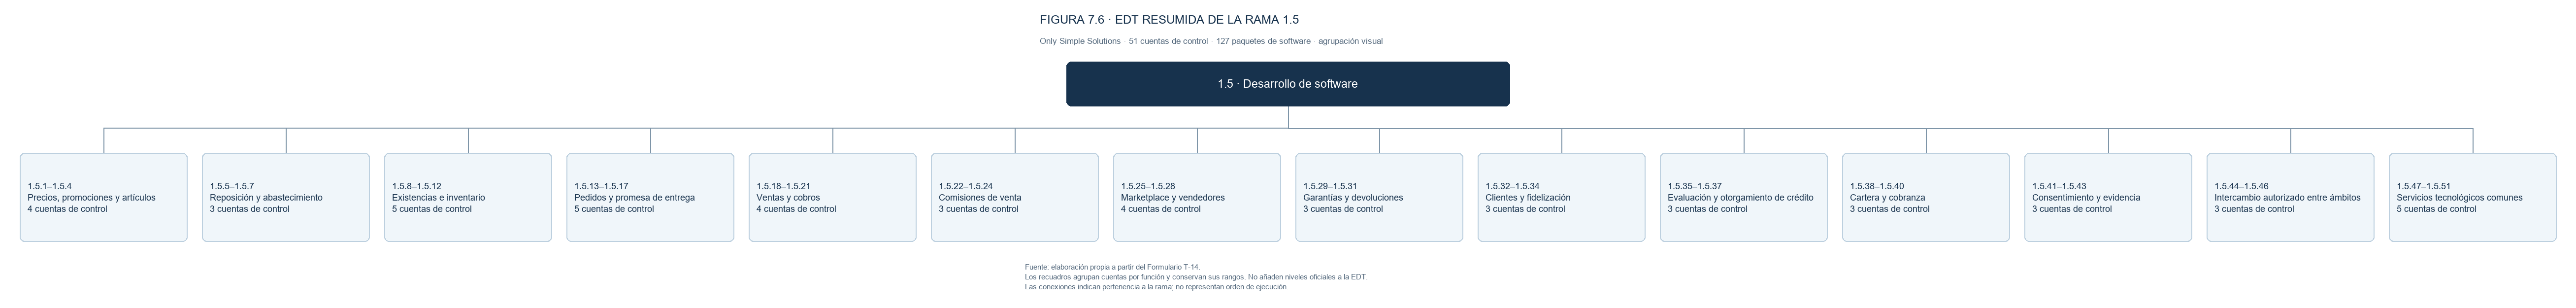
\includegraphics[width=\linewidth,height=\textheight,keepaspectratio]{figuras/sd07-figuras/sd07-edt1.5.png}
\raggedright\textbf{Fuente:} Elaboración propia a partir del Formulario T-14.
\end{minipage}
\end{center}


El trabajo parte de los requerimientos y de las decisiones de arquitectura. Incluye la construcción de las funciones y las comprobaciones necesarias antes de presentar cada entrega a las pruebas de la etapa. Los paquetes se distribuyen según el alcance de la Etapa 1 y la Etapa 2; algunas cuentas contemplan una entrega inicial y una ampliación posterior. Esa distribución se conserva en el T-14 y evita interpretar que todas las funciones estarán disponibles desde la primera puesta en servicio.

La rama entrega software cuyo comportamiento debe coincidir con las reglas aprobadas y contar con evidencia de calidad. Para utilizarlo se necesitan también las conexiones de la rama 1.6, los datos preparados en la 1.7 y los controles de seguridad correspondientes. Esta relación explica por qué terminar de programar una función es una parte del trabajo necesario para ponerla en operación. La aceptación considera el funcionamiento de la solución integrada.

\subsubsection{7.1.3.6 Integraciones (EDT 1.6)}

Las integraciones permiten que los sistemas intercambien información para completar una operación del negocio. En Ancoa, el proyecto debe abordar una red de plataformas y conexiones existentes (Multitiendas Ancoa S.A., 2026, Caso 09, cap. 5, p. 13). Antes de modificar esos intercambios se documenta qué información circula, quién la envía y quién la recibe. El catálogo de interfaces reúne esas conexiones y sus reglas; una interfaz es el medio acordado para que dos sistemas se comuniquen.

La Figura 7.7 presenta las 7 cuentas de control de esta rama, alineadas en un mismo nivel bajo el entregable principal.

\begin{center}
\begin{minipage}{\linewidth}
\centering
\ossFigCaption{EDT resumida de la rama 1.6}\label{fig:7-7}
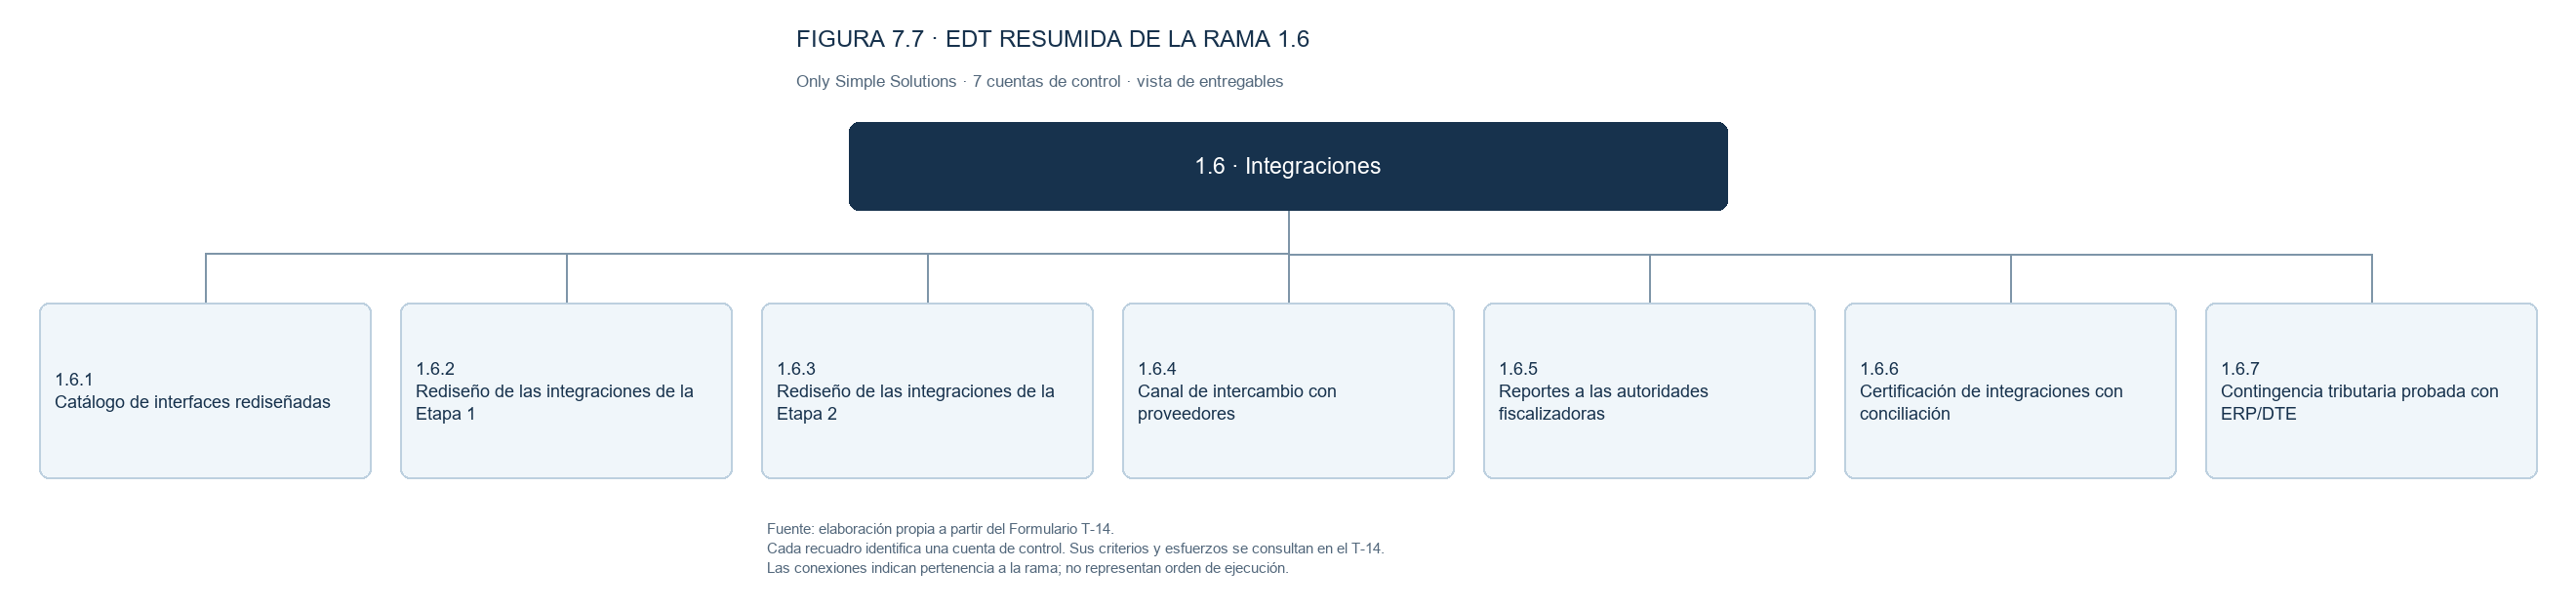
\includegraphics[width=\linewidth,height=\textheight,keepaspectratio]{figuras/sd07-figuras/sd07-edt1.6.png}
\raggedright\textbf{Fuente:} Elaboración propia a partir del Formulario T-14.
\end{minipage}
\end{center}

Esta rama desarrolla las conexiones de ambas etapas y comprueba su comportamiento de principio a fin. Incluye intercambios relacionados con precios, existencias y crédito, además de los previstos para pedidos, proveedores y otros servicios. También contempla los reportes a las entidades fiscalizadoras y las pruebas de contingencia de los documentos tributarios. Las reglas de intercambio especifican cómo deben interpretarse los datos para que el sistema receptor conserve su significado.

La verificación compara la información entre los sistemas que participan. Esta conciliación permite detectar diferencias que podrían dejar una operación registrada de forma distinta en cada plataforma. El resultado esperado es un conjunto de conexiones documentadas y probadas, con evidencia que permita explicar las diferencias encontradas y comprobar su tratamiento. Su entrega se coordina con el software de cada etapa y con los ensayos de funcionamiento conjunto.

\subsubsection{7.1.3.7 Migración y saneamiento de datos (EDT 1.7)}

La nueva solución necesita recibir información que ya existe en las plataformas de Ancoa. Esta rama prepara ese traslado y revisa la calidad de los datos antes de utilizarlos. El saneamiento trata problemas como duplicados o registros inconsistentes. La migración mueve la información al destino previsto, mientras que la conciliación compara ambos lados para comprobar que el traslado conserva los datos y los saldos que corresponden.

La Figura 7.8 presenta las 12 cuentas de control de esta rama, alineadas en un mismo nivel bajo el entregable principal.

\begin{center}
\begin{minipage}{\linewidth}
\centering
\ossFigCaption{EDT resumida de la rama 1.7}\label{fig:7-8}
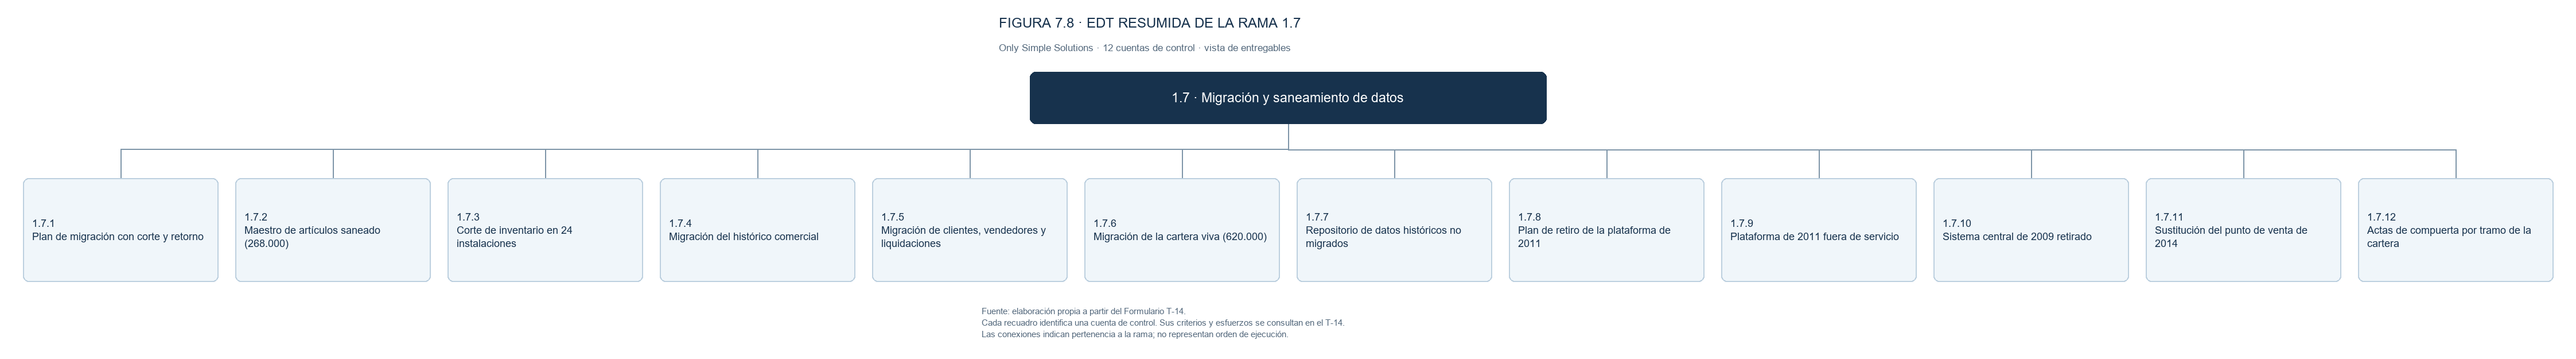
\includegraphics[width=\linewidth,height=\textheight,keepaspectratio]{figuras/sd07-figuras/sd07-edt1.7.png}
\raggedright\textbf{Fuente:} Elaboración propia a partir del Formulario T-14.
\end{minipage}
\end{center}

El trabajo abarca artículos, inventario e históricos comerciales, además de la información de clientes y la cartera de crédito. Cada conjunto requiere controles propios. En la cartera, las actas por tramo dejan evidencia de lo revisado antes de continuar; en el inventario, el corte y la conciliación deben coordinarse con la actividad de las instalaciones. El plan de migración también define cómo retornar si una ejecución presenta problemas y qué información histórica permanecerá disponible en un repositorio de consulta.

La rama contempla el retiro de plataformas cuando se hayan cumplido las condiciones de sustitución y resguardo. Algunos retiros se extienden al período de operación, según el calendario del T-14. Por ello, el resultado incluye tanto datos utilizables en la nueva solución como evidencia de la transición y del cierre de los sistemas sustituidos. La preparación se coordina con las integraciones y la implantación para evitar que cada equipo trabaje con versiones incompatibles de la información.

\subsubsection{7.1.3.8 Seguridad, identidad y cumplimiento (EDT 1.8)}

Esta rama protege la información y establece quién puede acceder a ella o ejecutar una acción. Su propósito es que los permisos correspondan a las responsabilidades de cada persona y que los datos sensibles cuenten con controles adecuados. La separación entre el negocio comercial y el emisor de crédito orienta estas definiciones (Multitiendas Ancoa S.A., 2026, Caso 09, cap. 13, núm. 13.3, condición 7, p. 30). Los controles contemplan además la separación de funciones dentro de los procesos financieros.

La Figura 7.9 presenta las 8 cuentas de control de esta rama, alineadas en un mismo nivel bajo el entregable principal.

\begin{center}
\begin{minipage}{\linewidth}
\centering
\ossFigCaption{EDT resumida de la rama 1.8}\label{fig:7-9}
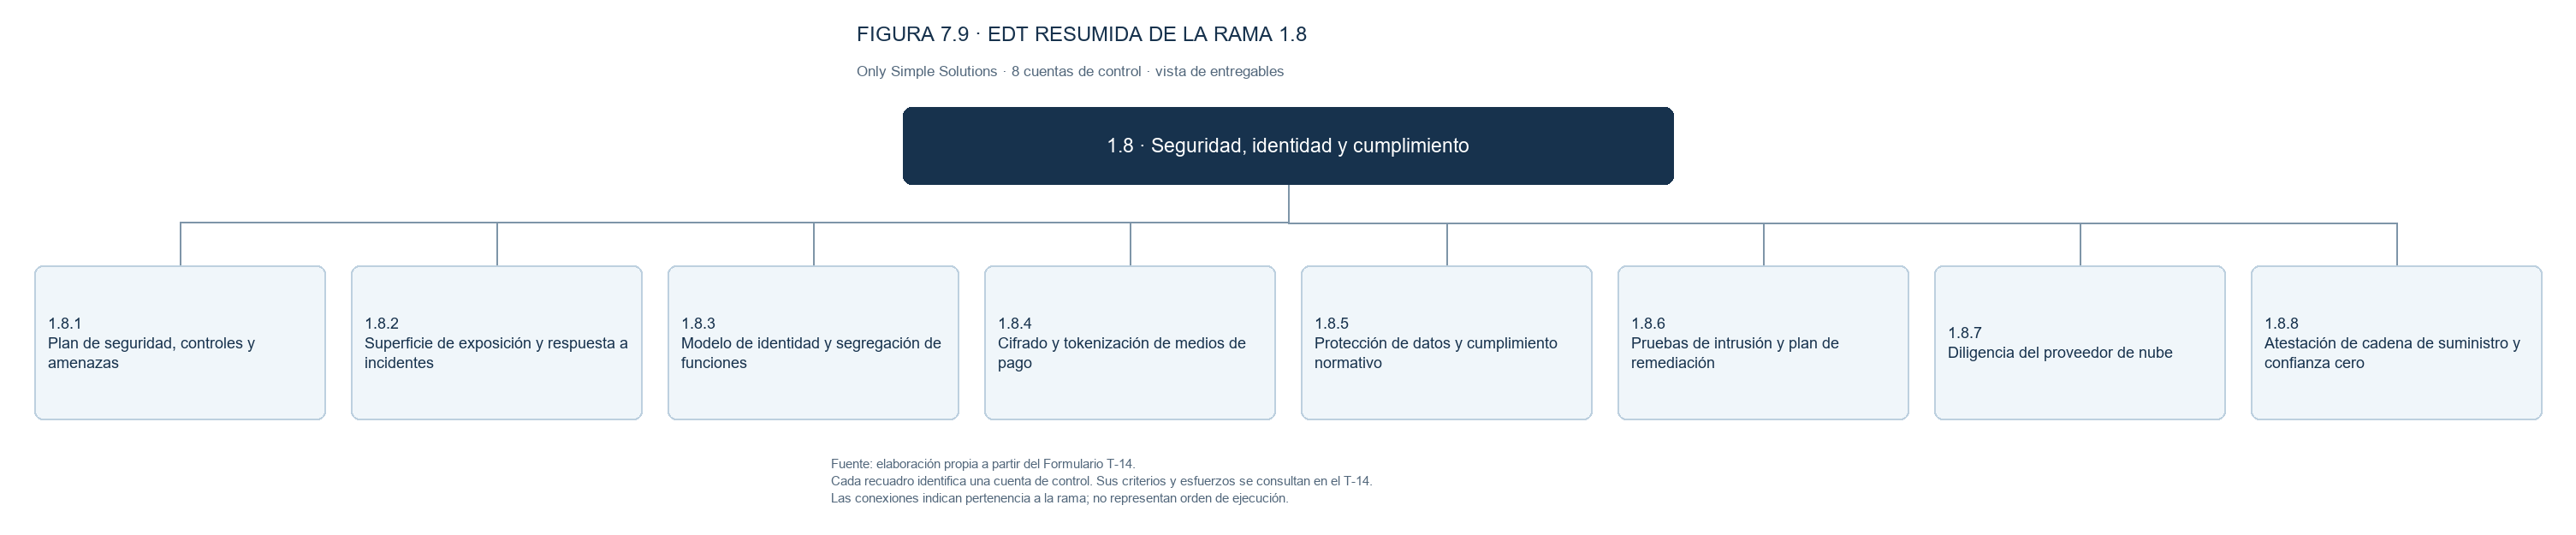
\includegraphics[width=\linewidth,height=\textheight,keepaspectratio]{figuras/sd07-figuras/sd07-edt1.8.png}
\raggedright\textbf{Fuente:} Elaboración propia a partir del Formulario T-14.
\end{minipage}
\end{center}

El trabajo comprende el análisis de amenazas, las medidas de protección de datos y la preparación de la respuesta a incidentes. Una amenaza es una situación que podría comprometer la información o el servicio; identificarla permite definir controles y procedimientos de respuesta. La rama también incluye la evaluación de controles del proveedor de nube y de los componentes incorporados a la solución. Las pruebas de intrusión buscan debilidades mediante intentos controlados de vulnerar las protecciones.

Los entregables reúnen las medidas implementadas y la evidencia de su comprobación. Los hallazgos detectados deben tratarse según su gravedad y verificarse de nuevo antes de la aceptación correspondiente. Este trabajo comienza durante el diseño y se coordina con la infraestructura, el desarrollo y las pruebas de cada etapa. La rama aporta los controles y su evidencia; el seguimiento cotidiano durante el servicio se articula con la operación.

\subsubsection{7.1.3.9 Calidad, pruebas y certificación (EDT 1.9)}

La calidad se comprueba mediante pruebas planificadas y resultados observables. Esta rama define qué se revisará, con qué condiciones y qué evidencia permitirá decidir si una entrega cumple lo comprometido. Las pruebas funcionales verifican tareas del negocio. Las pruebas de desempeño revisan cómo responde el sistema ante la carga prevista, y las de recuperación comprueban su comportamiento frente a interrupciones.

La Figura 7.10 presenta las 12 cuentas de control de esta rama, alineadas en un mismo nivel bajo el entregable principal.

\begin{center}
\begin{minipage}{\linewidth}
\centering
\ossFigCaption{EDT resumida de la rama 1.9}\label{fig:7-10}
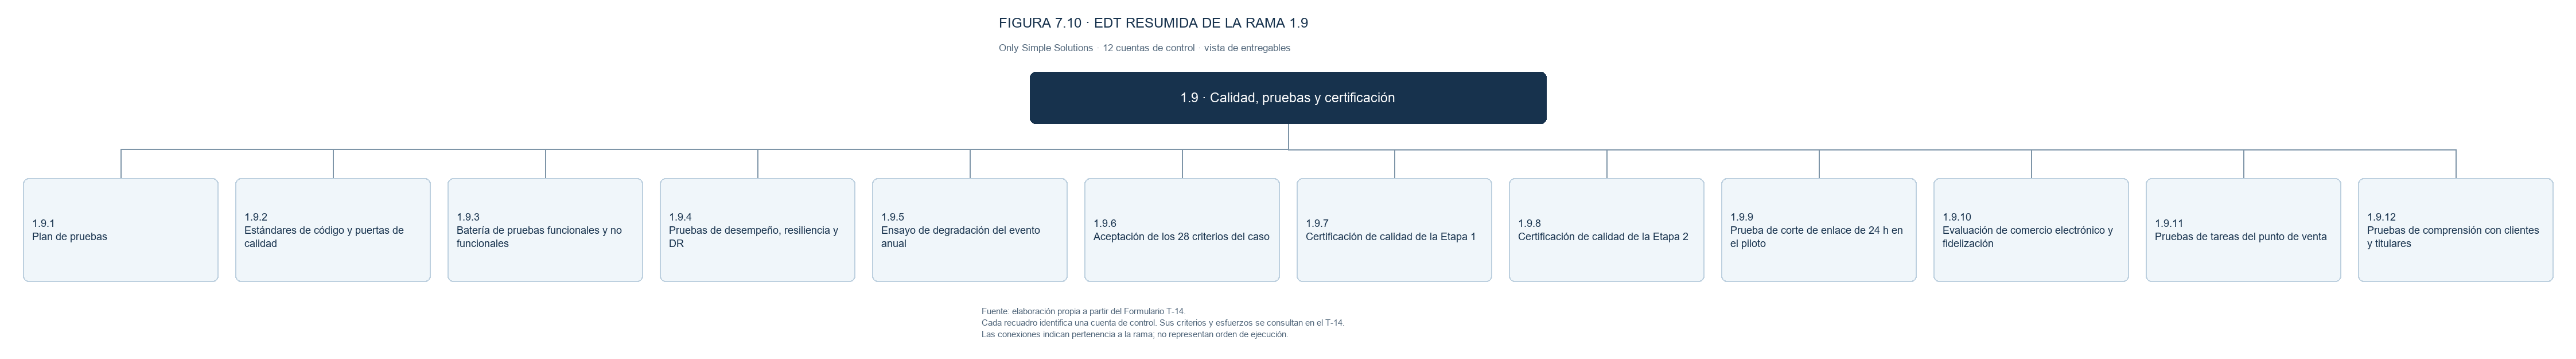
\includegraphics[width=\linewidth,height=\textheight,keepaspectratio]{figuras/sd07-figuras/sd07-edt1.9.png}
\raggedright\textbf{Fuente:} Elaboración propia a partir del Formulario T-14.
\end{minipage}
\end{center}

El trabajo incluye ensayos del punto de venta, pérdida de conexión y funcionamiento bajo alta demanda. También considera la comprensión de la información por parte de usuarios y clientes. Un sistema puede ejecutar una operación y aun así presentar dificultades de uso; estas comprobaciones permiten identificar ambos tipos de problema. Cuando se detecta un defecto, su corrección debe volver a probarse para demostrar que resolvió el hallazgo.

La certificación reúne los resultados de las pruebas exigidas para cada etapa. Esta evidencia se prepara antes de su marcha blanca y permite revisar si la solución está en condiciones de avanzar. Esta rama se concentra en demostrar el cumplimiento técnico y funcional, mientras que la 1.12 registra los resultados de la operación supervisada y la aceptación formal. Los criterios y umbrales específicos permanecen en el diccionario del T-14 y en los documentos de calidad relacionados.

\subsubsection{7.1.3.10 Innovaciones (EDT 1.10)}

Esta rama reúne cinco mejoras que amplían los servicios de Ancoa y la forma en que sus clientes y trabajadores los utilizan. Abarca el retiro de pedidos, el conteo de inventario, la búsqueda de productos, la publicidad para proveedores y la atención en probadores. La EDT identifica el trabajo necesario para poner cada mejora en funcionamiento y comprobar su aporte. El Subdocumento 13 desarrolla su justificación, tecnología, indicadores, riesgos e impacto económico; aquí se resume qué hace cada una y para qué se incorpora.

La Figura 7.11 muestra las cinco cuentas reservadas para innovaciones. Su definición y alcance detallado están en el Subdocumento 13.

\begin{center}
\begin{minipage}{\linewidth}
\centering
\ossFigCaption{EDT resumida de la rama 1.10}\label{fig:7-11}
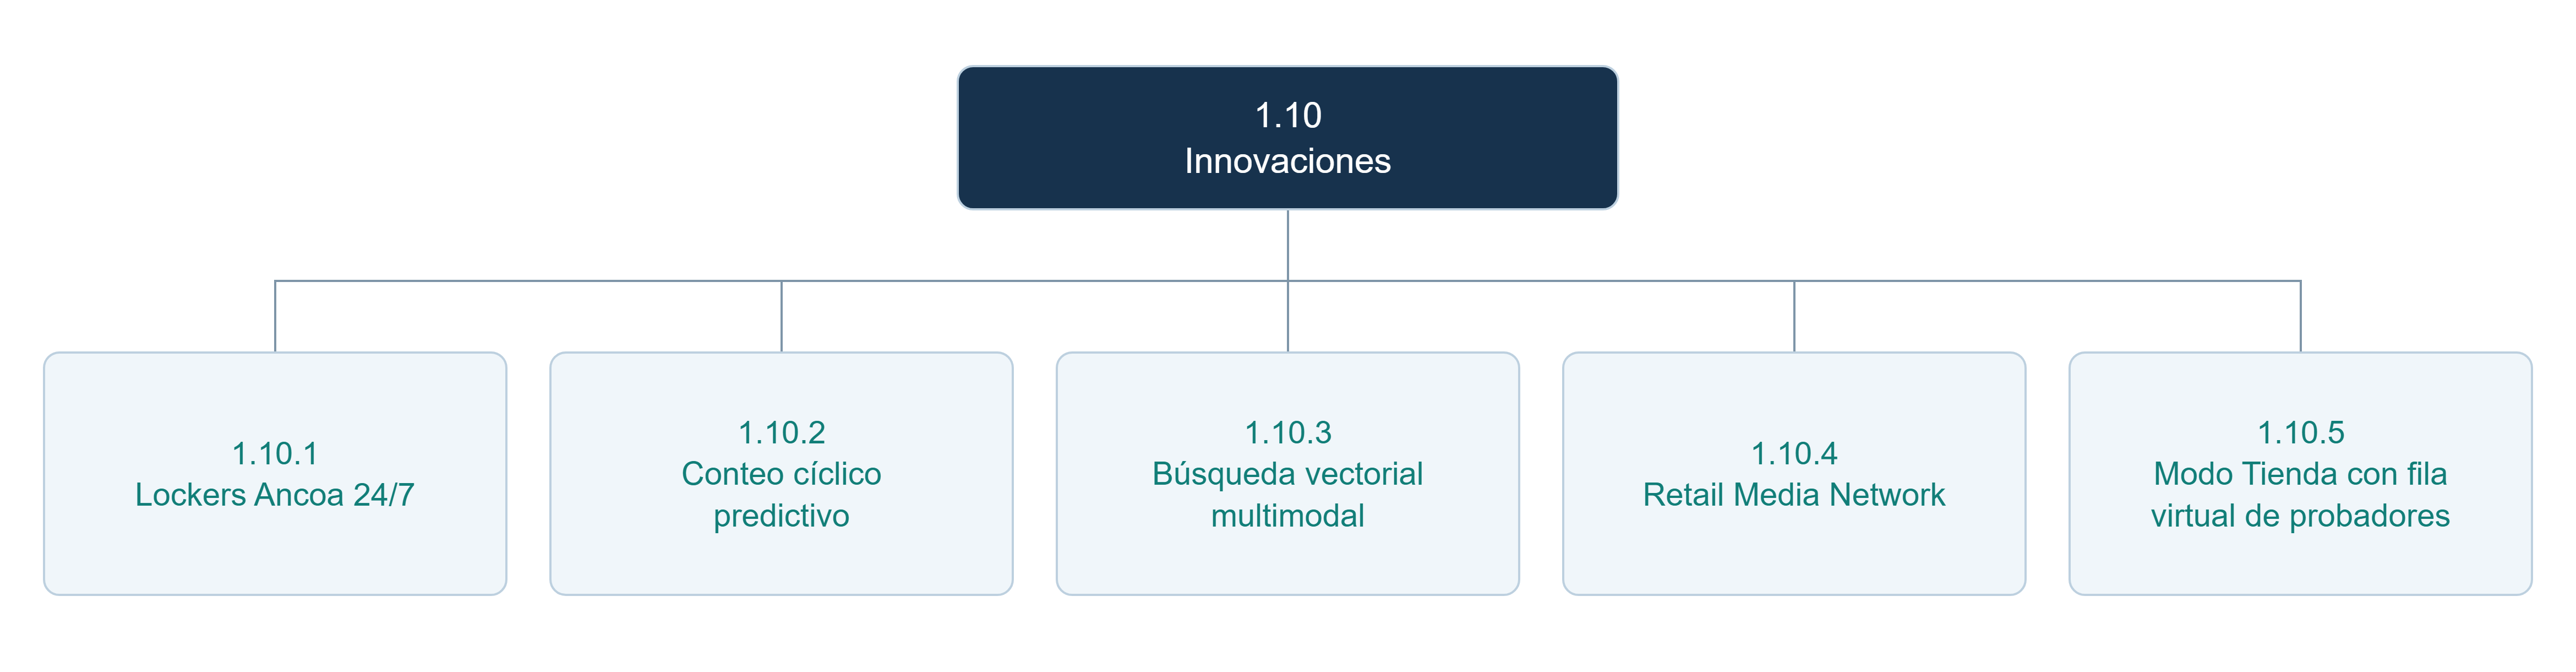
\includegraphics[width=\linewidth,height=\textheight,keepaspectratio]{figuras/sd07-figuras/sd07-edt1.10.png}
\raggedright\textbf{Fuente:} Elaboración propia a partir del Formulario T-14.
\end{minipage}
\end{center}

Lockers Ancoa 24/7 ofrece casilleros electrónicos para retirar compras sin pasar por el mesón. Se incorporan para ampliar los horarios de retiro y facilitar la entrega de pedidos.
El conteo cíclico predictivo es una herramienta que identifica los productos con mayor riesgo de presentar diferencias de inventario. Se incorpora para orientar los conteos y aprovechar mejor el tiempo del personal.
La búsqueda vectorial multimodal permite encontrar productos mediante fotografías o descripciones en lenguaje cotidiano. Se incorpora para facilitar la búsqueda y mejorar la experiencia de compra.
Retail Media Network es un servicio de publicidad para que los proveedores promocionen productos en el canal digital de Ancoa. Se incorpora para generar ingresos publicitarios.
El Modo Tienda con fila virtual de probadores permite solicitar un turno sin permanecer físicamente en la fila. Se incorpora para organizar la atención y mejorar la experiencia dentro de la tienda.

\subsubsection{7.1.3.11 Implantación y despliegue (EDT 1.11)}

La implantación prepara la solución para su uso en las dependencias de Ancoa. Esta rama coordina la configuración de los sitios y la publicación de las versiones que utilizará cada etapa. El plan identifica cómo realizar el cambio y cómo volver a la situación anterior si aparecen fallas. Este retorno debe ensayarse, porque durante una intervención pueden existir operaciones que es necesario conservar y conciliar.

La Figura 7.12 presenta las 4 cuentas de control de esta rama, alineadas en un mismo nivel bajo el entregable principal.

\begin{center}
\begin{minipage}{\linewidth}
\centering
\ossFigCaption{EDT resumida de la rama 1.11}\label{fig:7-12}
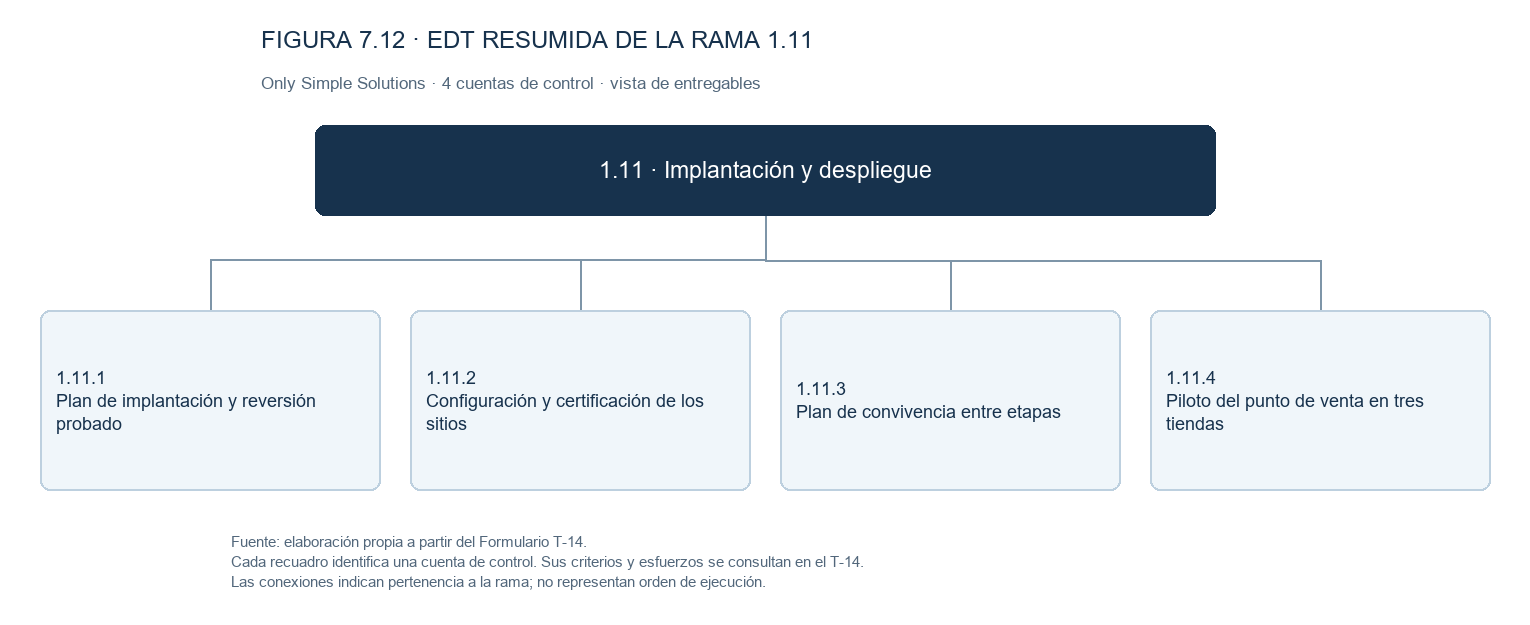
\includegraphics[width=\linewidth,height=0.75\textheight,keepaspectratio]{figuras/sd07-figuras/sd07-edt1.11.png}
\raggedright\textbf{Fuente:} Elaboración propia a partir del Formulario T-14.
\end{minipage}
\end{center}

El piloto técnico permite comprobar el funcionamiento en un entorno controlado de las tiendas seleccionadas. Durante ese ensayo, la venta oficial continúa en los sistemas vigentes. Sus resultados aportan evidencia para ajustar los procedimientos antes del despliegue correspondiente. La rama también prepara la convivencia entre etapas, con reglas que eviten registrar dos veces una misma operación o mantener datos contradictorios entre versiones.

El resultado esperado es una preparación de los sitios y un procedimiento de despliegue cuya ejecución y retorno hayan sido comprobados. El plan respeta las restricciones de intervención y los períodos de congelamiento (Multitiendas Ancoa S.A., 2026, Caso 09, cap. 13, núm. 13.2, p. 29; núm. 13.3, condición 3, p. 30). La puesta en producción se realiza después de cumplir las condiciones de marcha blanca y aceptación; la instalación técnica por sí sola no habilita ese paso. El T-18 desarrolla la estrategia y sus controles, mientras que el apartado 7.3 presenta su ubicación en el calendario.

\subsubsection{7.1.3.12 Resultados de las marchas blancas y aceptación por etapa (EDT 1.12)}

La marcha blanca permite observar la solución en funcionamiento real bajo supervisión antes de aceptar cada etapa. Su plan define qué se medirá, qué evidencia se recogerá y qué condiciones deben cumplirse al finalizar. Durante ese período se registran los problemas encontrados y sus correcciones. Los informes permiten evaluar si el comportamiento observado es consistente con los compromisos de la propuesta.

La Figura 7.13 presenta las 7 cuentas de control de esta rama, alineadas en un mismo nivel bajo el entregable principal.

\begin{center}
\begin{minipage}{\linewidth}
\centering
\ossFigCaption{EDT resumida de la rama 1.12}\label{fig:7-13}
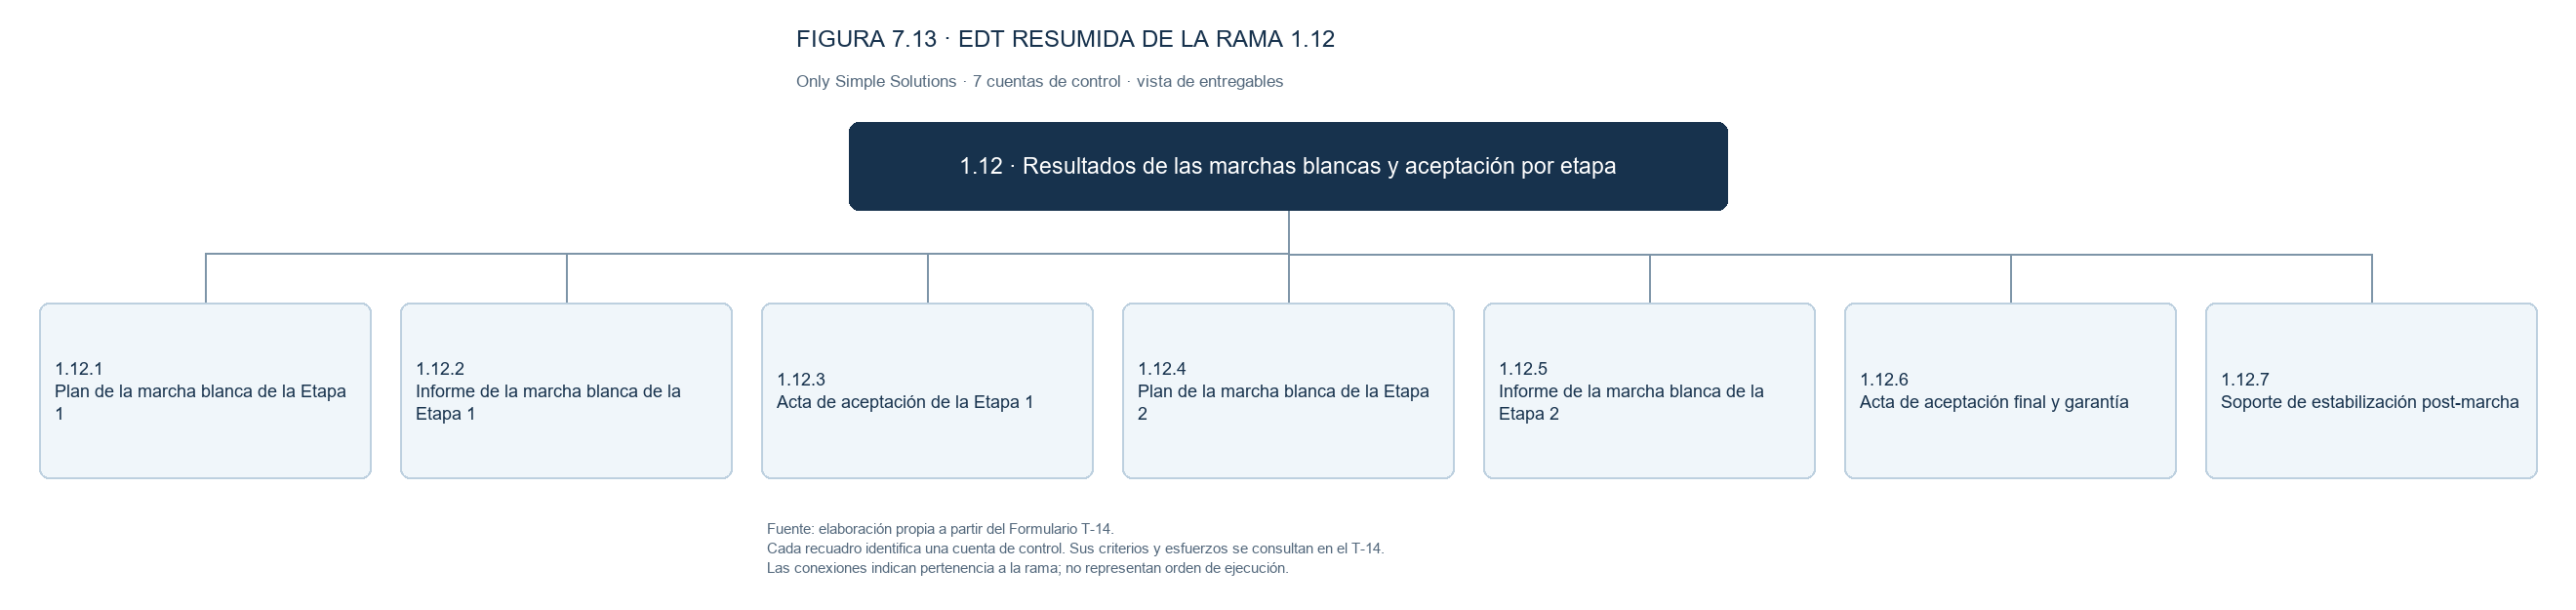
\includegraphics[width=\linewidth,height=\textheight,keepaspectratio]{figuras/sd07-figuras/sd07-edt1.12.png}
\raggedright\textbf{Fuente:} Elaboración propia a partir del Formulario T-14.
\end{minipage}
\end{center}

El cierre considera las condiciones del artículo 17.3. Debe acreditarse la ausencia de incidentes críticos y altos, el volumen real comprometido durante las últimas cuatro semanas y el cumplimiento sostenido de disponibilidad y respuesta en ese mismo período. También se exige conciliación sin diferencias no explicadas, personal capacitado y certificado, y el acta de aceptación firmada. El T-18 desarrolla estas condiciones y la evidencia requerida.

Esta rama entrega los planes e informes de ambas marchas blancas, junto con sus actas de aceptación y el seguimiento de estabilización posterior. El cumplimiento se demuestra con los resultados registrados; llegar al mes previsto no basta para dar la etapa por aceptada. La información de las pruebas, la capacitación y la migración alimenta esta decisión. Después del cierre, los mecanismos de seguimiento permiten tratar las incidencias de la adaptación inicial y coordinar su atención con la operación.

\subsubsection{7.1.3.13 Gestión del cambio y capacitación (EDT 1.13)}

La incorporación de una solución modifica tareas habituales y requiere preparar a quienes las realizan. Esta rama identifica las necesidades de aprendizaje según el rol y organiza la capacitación para que cada persona pueda utilizar las funciones que le corresponden. La preparación debe considerar tanto al personal de las tiendas como a quienes administrarán y sostendrán técnicamente el servicio.

La Figura 7.14 presenta las 5 cuentas de control de esta rama, alineadas en un mismo nivel bajo el entregable principal.

\begin{center}
\begin{minipage}{\linewidth}
\centering
\ossFigCaption{EDT resumida de la rama 1.13}\label{fig:7-14}
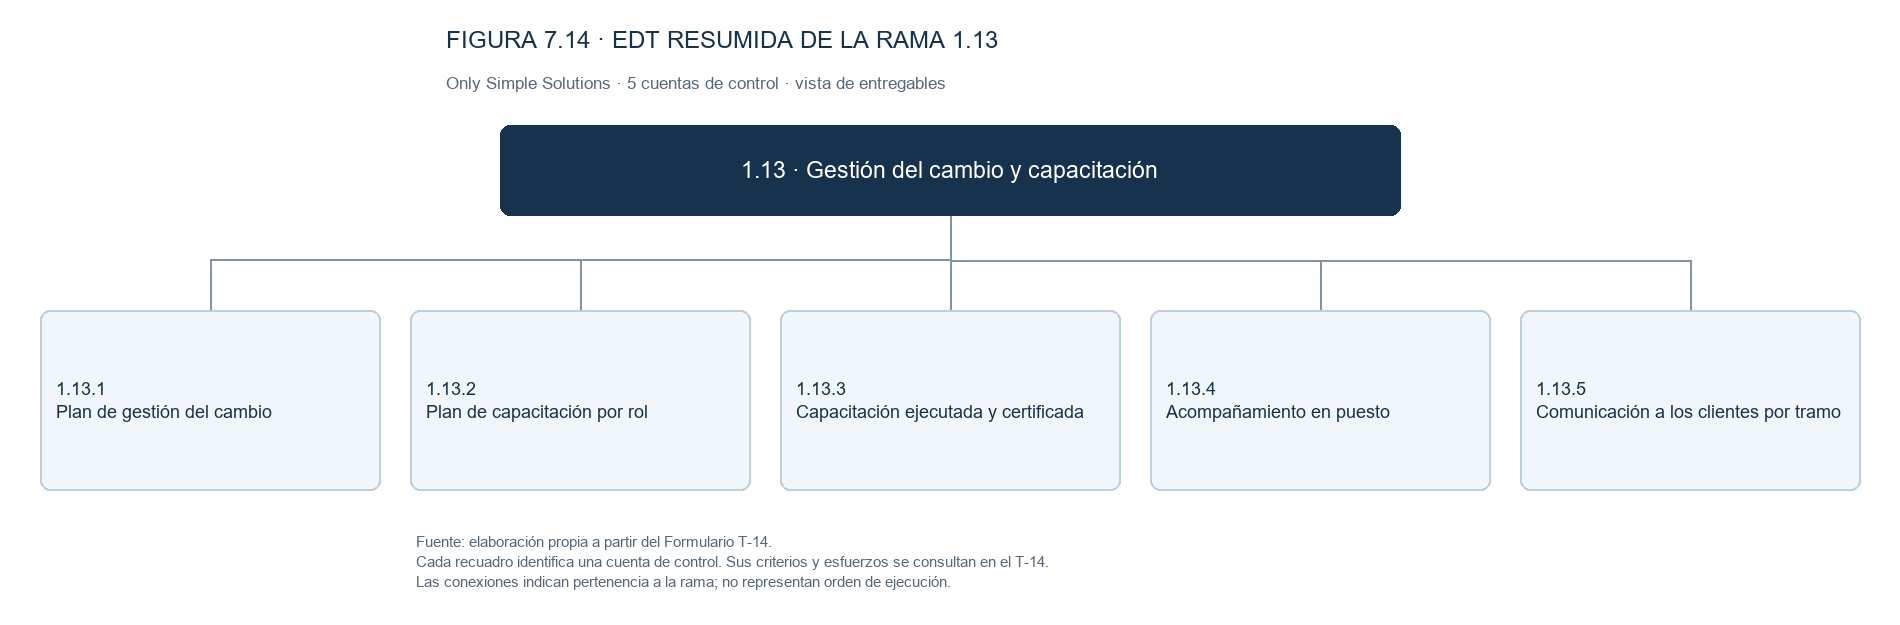
\includegraphics[width=\linewidth,height=\textheight,keepaspectratio]{figuras/sd07-figuras/sd07-edt1.13.png}
\raggedright\textbf{Fuente:} Elaboración propia a partir del Formulario T-14.
\end{minipage}
\end{center}

El trabajo incluye planes de capacitación, materiales editables en español y evaluaciones que permitan comprobar el aprendizaje. También contempla acompañamiento en el puesto, donde pueden aparecer dudas que no se detectaron durante una sesión de formación. Ese apoyo cobra relevancia para el personal nuevo, temporal o externo que participa en la operación. La formación de esos grupos y la comunicación a los clientes durante la migración de cartera responden a condiciones del caso (Multitiendas Ancoa S.A., 2026, Caso 09, cap. 13, núm. 13.3, condiciones 5 y 8, p. 30). Las comunicaciones se coordinan con los tramos de migración previstos.

Los resultados se expresan en registros de formación y certificación, materiales disponibles y evidencia del acompañamiento. La preparación de los usuarios necesarios para la marcha blanca debe completarse antes de su participación. Las certificaciones de cierre se documentan conforme al plan de cada etapa. Esta rama conecta el trabajo técnico con su uso cotidiano y aporta a la aceptación evidencia de que las personas cuentan con la habilitación requerida para desempeñar sus funciones.

\subsubsection{7.1.3.14 Documentación, transferencia y reversibilidad (EDT 1.14)}

Esta rama conserva el conocimiento necesario para comprender y administrar la solución durante su vida contractual. La documentación describe las funciones y los componentes técnicos, mientras que los manuales y la base de conocimiento apoyan las tareas habituales de operación. Mantener estos materiales al día permite que los cambios implementados queden reflejados en la información que utiliza el personal.

La Figura 7.15 presenta las 7 cuentas de control de esta rama, alineadas en un mismo nivel bajo el entregable principal.

\begin{center}
\begin{minipage}{\linewidth}
\centering
\ossFigCaption{EDT resumida de la rama 1.14}\label{fig:7-15}
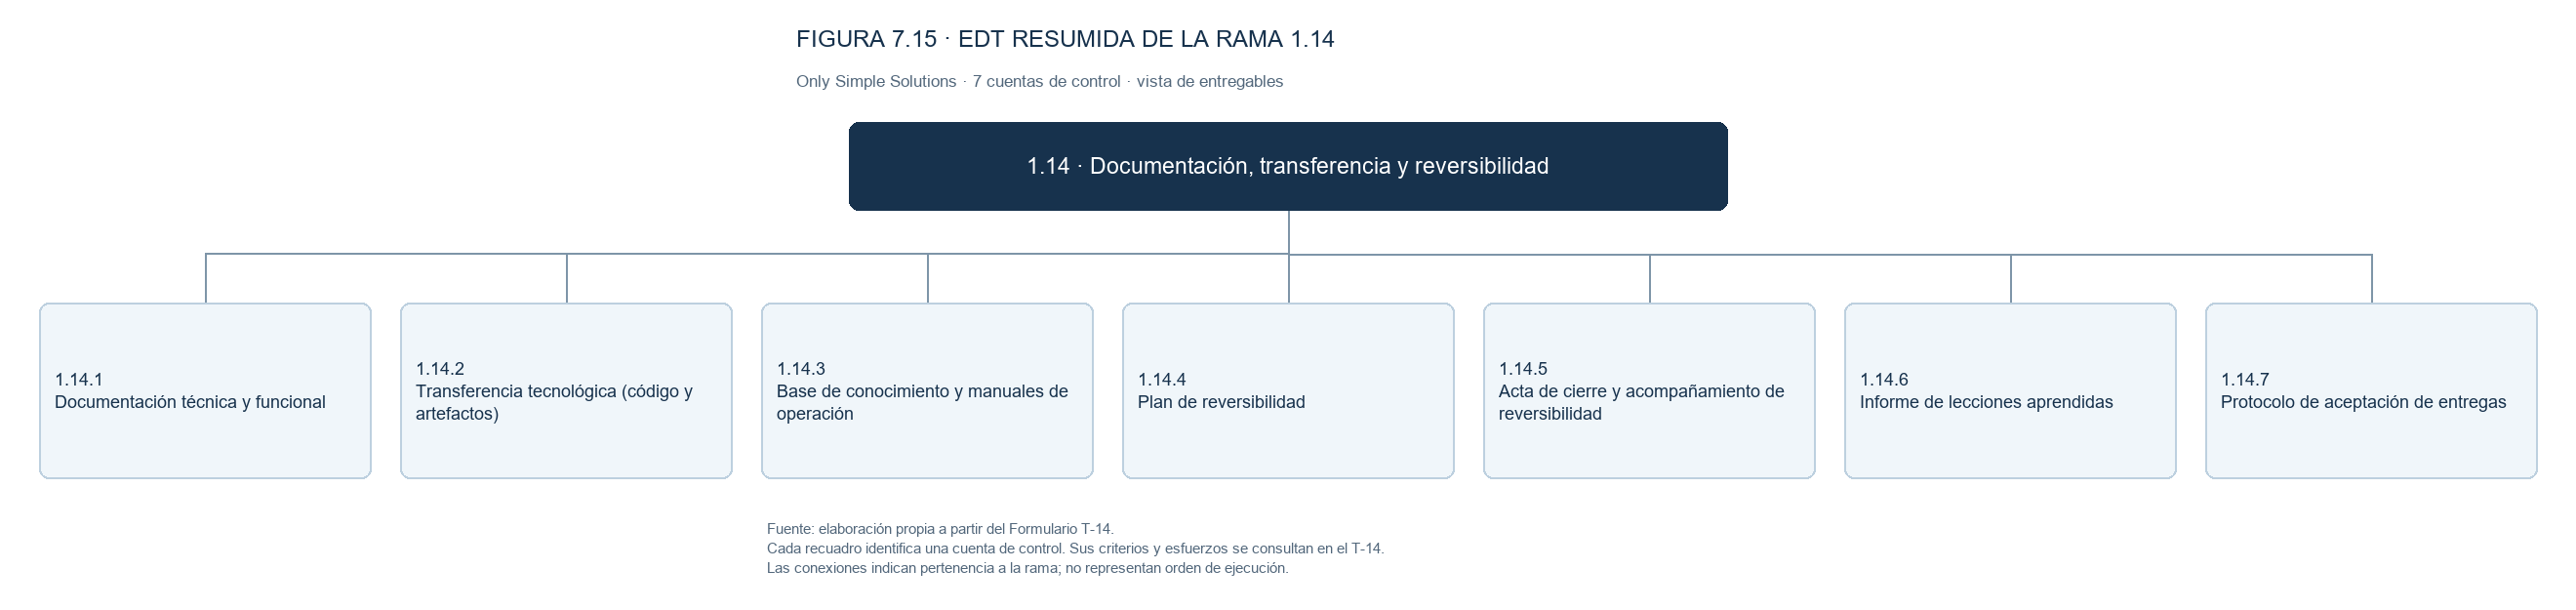
\includegraphics[width=\linewidth,height=\textheight,keepaspectratio]{figuras/sd07-figuras/sd07-edt1.14.png}
\raggedright\textbf{Fuente:} Elaboración propia a partir del Formulario T-14.
\end{minipage}
\end{center}

La transferencia comprende el código y los elementos necesarios para reconstruir y desplegar la solución de acuerdo con las entregas establecidas. La reversibilidad prepara el traspaso del servicio y de los datos al término del contrato. Su plan debe explicar cómo realizar esa transición y mantener información utilizable por quien reciba el servicio. Esta preparación se desarrolla durante el contrato y se actualiza conforme a sus condiciones.

Los entregables incluyen documentación vigente, procedimientos y registros del traspaso final. También se reúnen las lecciones aprendidas y el acta de cierre. La rama se alimenta de los cambios realizados por desarrollo, infraestructura y operación, por lo que requiere coordinación con esos equipos. Su propósito es que Ancoa disponga de información suficiente para recibir la solución y dar continuidad a su administración una vez terminado el servicio contratado.

El traspaso final se prepara en M48–56 y su acompañamiento se programa en M54–56, con al menos 90 días efectivos antes del cierre. Se conservan las 64 HH de la cuenta 1.14.5; el T-15 distribuye esa dedicación y el anexo CPM distingue la holgura total del margen que queda disponible en las fechas programadas.

\subsubsection{7.1.3.15 Operación y soporte (EDT 1.15)}

La operación sostiene el funcionamiento de la solución durante los 36 meses comprendidos entre M21 y M56. Esta rama reúne la atención a los usuarios, el tratamiento de incidentes y la administración de los medios tecnológicos. La mesa de servicio recibe los problemas y los deriva al nivel de atención que corresponde según su naturaleza. El seguimiento debe permitir conocer su estado y comprobar los tiempos de respuesta y resolución comprometidos.

La Figura 7.16 presenta las 6 cuentas de control de esta rama, alineadas en un mismo nivel bajo el entregable principal.

\begin{center}
\begin{minipage}{\linewidth}
\centering
\ossFigCaption{EDT resumida de la rama 1.15}\label{fig:7-16}
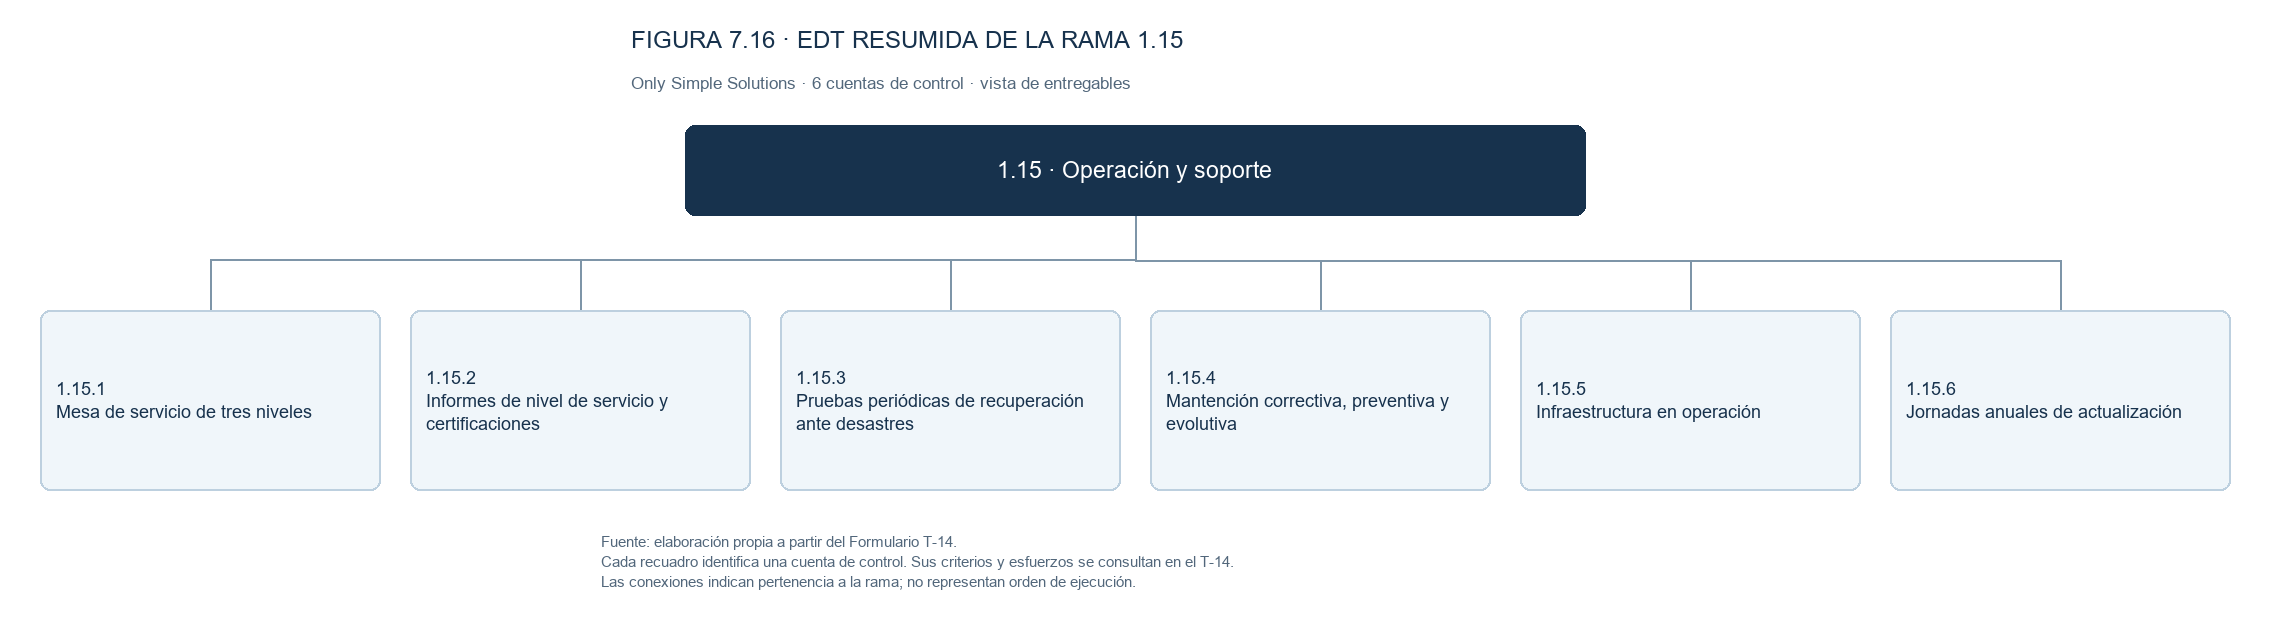
\includegraphics[width=\linewidth,height=\textheight,keepaspectratio]{figuras/sd07-figuras/sd07-edt1.15.png}
\raggedright\textbf{Fuente:} Elaboración propia a partir del Formulario T-14.
\end{minipage}
\end{center}

El mantenimiento correctivo resuelve fallas; el preventivo atiende condiciones que podrían causarlas, y el evolutivo incorpora los cambios previstos en su plan. La administración de infraestructura revisa la capacidad y disponibilidad del servicio. También se realizan pruebas periódicas de recuperación para comprobar que los procedimientos y respaldos siguen siendo utilizables. Las jornadas de actualización apoyan al personal nuevo y a quienes deben adaptarse a cambios durante la operación.

Los informes de nivel de servicio reúnen las mediciones y la evidencia de cumplimiento. Así, Ancoa puede evaluar el funcionamiento con registros del período, además de conocer las incidencias y acciones realizadas. Los subdocumentos de operación desarrollan estas obligaciones y los planes relacionados. La EDT identifica sus entregables; la dotación por rol y la cobertura de atención deben completarse en los documentos de equipo y recursos, porque una asignación de horas por sí sola no demuestra capacidad suficiente para sostener el servicio.


\section{7.2 Plan de trabajo}\label{plan-de-trabajo}

El plan organiza las quince ramas de la EDT en once frentes y mantiene el despliegue híbrido, las dos etapas de implementación y los 36 meses de operación. El Formulario T-14 detalla las cuentas, sus entregas y ventanas; el T-15 calcula su carga mensual. La segregación de los dominios Retail y Emisor se conserva durante la construcción, migración y operación. La coordinación de iteraciones y aceptación por entregables se articula con el Capítulo 6.

\subsection{7.2.1 Secuenciamiento y estimación}

La línea base inicial se acepta en H1, mes 2. La arquitectura, el modelo de datos y el plan de seguridad se aprueban en H2, mes 4; la infraestructura híbrida y los cinco ambientes operativos se entregan en H3, mes 6. Los ambientes se habilitan progresivamente para diseño, pruebas de componentes y el piloto técnico. La entrega integrada de H3 permite la integración final; no significa que todo el desarrollo deba esperar hasta ese mes; las entregas mantienen su trazabilidad con el Formulario E-25 y el requisito RT-04.01.

El software E1 llega a pruebas con QA superado en H4, mes 10, y se certifica en H5, mes 12. La marcha blanca ocupa M13-15 y la aceptación productiva H7 ocurre en M16. E2 comienza en M13 con análisis y diseño, cuya línea base se aprueba en H8, mes 14. La construcción dependiente se concentra en M15-17, entrega para pruebas en H9 y se certifica en H10, mes 18. La marcha blanca M19-20 antecede a H12, mes 21. Las cuentas que abarcan ambos alcances tienen entregas parciales separadas.

La Tabla 7.2 resume el esfuerzo planificado por ámbito. El T-14 presenta el detalle por cuenta y por los 127 paquetes de software.

\begin{longtable}{p{0.55\linewidth}p{0.14\linewidth}p{0.2\linewidth}}
\caption{Esfuerzo de la base de planificación.}\label{tab:7-2}\\
\toprule\noalign{}
\textbf{Ámbito} & \textbf{Cuentas} & \textbf{Horas hombre} \\
\midrule
\endhead
\bottomrule
\multicolumn{3}{@{}l}{\rule{0pt}{3.2ex}\textbf{Fuente:} Elaboración propia a partir de las cuentas planificadas del T-14.} \\
\endlastfoot
Desarrollo de software, rama 1.5 & 51 & 12.116 \\
Ramas distintas del software & 113 & 28.830 \\
Total & 164 & 40.946 \\
\end{longtable}

Las horas por paquete de software se concilian dentro de cada cuenta, distribuyendo los restos de redondeo sin cambiar la asignación de esa cuenta. La descomposición por roles, dedicaciones y cobertura de turnos debe conservar esos totales y demostrar los niveles de servicio en los subdocumentos 10 y 12. Una suma de horas no demuestra por sí sola una dotación suficiente.

\subsection{7.2.2 Organización del trabajo conforme al Capítulo 6}

La ejecución sigue Scrum para la construcción de software y Kanban para plataforma, soporte e incidencias, conforme a los apartados 6.1.3.3 y 6.2.1. Al comienzo de cada intervalo de dos meses, los responsables identifican los entregables del T-14 que contribuyen al siguiente hito y sus dependencias. Los sprints de dos semanas producen incrementos comprobables dentro de ese intervalo; no se fuerza una equivalencia exacta entre un mes calendario y dos sprints.

Una historia entra al sprint cuando tiene requisito y paquete asociados, criterios de aceptación, datos de prueba y dependencias resueltas. Las historias que cruzan la frontera Retail–Emisor requieren la revisión previa de seguridad y datos. El resultado terminado incluye código revisado, pruebas satisfactorias, documentación y evidencia, según 6.2.2 y 6.2.5. Las pruebas se ejecutan durante la construcción; las barras de certificación representan su cierre integrado y formal, no el comienzo de la verificación.

Los equipos de Retail, Emisor y plataforma conservan responsabilidades separadas. El frente de plataforma habilita ambientes, identidad, integración y observabilidad antes del trabajo dependiente. La reunión semanal resuelve impedimentos y el Comité de Proyecto quincenal revisa su efecto sobre los hitos. El avance se reconoce por entregables comprobados, con trazabilidad hacia la EDT, conforme a 6.1.3.5.

\subsection{7.2.3 Frentes de trabajo}

Los once frentes agrupan responsabilidades que avanzan en paralelo y entregan evidencia en los hitos contractuales. La Tabla 7.3 identifica su alcance temporal; las ventanas por cuenta mandan sobre este resumen.

\begin{longtable}{p{0.23\linewidth}p{0.12\linewidth}p{0.29\linewidth}p{0.24\linewidth}}
\caption{Frentes de trabajo.}\label{tab:7-3}\\
\toprule\noalign{}
\textbf{Frente} & \textbf{Ramas} & \textbf{Responsable principal} & \textbf{Ventana} \\
\midrule
\endhead
\bottomrule
\multicolumn{4}{@{}l}{\rule{0pt}{3.2ex}\textbf{Fuente:} Elaboración propia a partir de la EDT y del cronograma del T-14.} \\
\endlastfoot
Dirección y gobierno & 1.1 & Jefe de Proyecto & M1-56 \\
Levantamiento, alcance y arquitectura & 1.2, 1.3 & Líder Funcional / Arquitecto & M1-18, con entregas H1, H2 y H8 \\
Infraestructura híbrida & 1.4 & Arquitecto de Solución & M1-6, entrega H3 \\
Software & 1.5 & Líder de Desarrollo & E1 M1-12; E2 M13-18 \\
Integraciones y datos & 1.6, 1.7 & Líderes de Integración y Datos & M2-56, por entregas y retiros \\
Seguridad y cumplimiento & 1.8 & Encargado de Seguridad & M1-18, evidencia por etapa \\
Calidad y certificación & 1.9 & Líder de Calidad & M1-21, entregas H5 y H10 \\
Innovaciones & 1.10 & Arquitecto de Solución & E1 M5–15; E2 M13–20; seguimiento hasta M56 \\
Implantación, marchas blancas y cambio & 1.11-1.13 & Líder de Implantación y Cambio & M3-24, con tramos diferenciados \\
Documentación y reversibilidad & 1.14 & Jefe de Proyecto & M1-56 \\
Operación y soporte & 1.15 & Líder de Operación / SRE & M21-56 \\
\end{longtable}


La arquitectura y los controles de seguridad se entregan antes de los incrementos que dependen de ellos. Las pruebas acompañan la construcción y se cierran por etapa; no se acumulan hasta H12. La operación incluye pruebas de recuperación al menos semestrales, consistentes con el alcance del Subdocumento 3.

\subsection{7.2.4 Paralelización y sincronización entre etapas}

Durante M13-15 coexisten la marcha blanca E1 y el análisis, diseño e inicio de construcción E2. Durante M19-20 coexisten E1 en producción y la marcha blanca E2. El plan de convivencia de la cuenta 1.11.3 se prepara en M10-12, antes de comenzar el primer solapamiento. La conciliación identifica la fuente de verdad por entidad dentro de cada dominio; no mezcla los datos comerciales con los de la filial emisora.

El T-15 asigna el esfuerzo E2 únicamente desde M13. Los trabajos de gobierno y documentación permanecen transversales y su carga posterior a M21 se incluye en la curva de operación. El acta de aceptación final en M21 se mantiene en implementación; así se evita duplicar horas en el mes de transición.

El máximo de la implementación recalculada es 2.492,78 HH en M16. La conversión a 160 HH por persona-mes expresa capacidad equivalente, no número suficiente de profesionales por rol. El T-15 muestra las cargas de ambos solapamientos y distingue esta medida de la dotación nominal.

\subsubsection{7.2.4.1 Capacidad durante los solapamientos}

En M13–15, los responsables separan la capacidad de estabilización de E1 de la comprometida para análisis, diseño y construcción de E2. En M19–20, separan el soporte de E1 en producción de la marcha blanca E2. Según 6.2.7, cada equipo de desarrollo que participa en una marcha blanca reserva el 30 \% de su capacidad disponible para incidencias y estabilización. La reserva del 15 \% para deuda técnica de 6.2.3.3 se mantiene sobre la misma base; cuando ambas coinciden, el máximo comprometible para otras historias es el 55 \%. Un trabajo no se imputa simultáneamente a las dos reservas.

Estas proporciones son reglas de asignación de capacidad y no recargos sobre las 40.946 HH planificadas. El T-15 establece su conciliación por equipo, rol e intervalo. Si la carga supera la capacidad disponible, el jefe de proyecto resuelve la asignación antes de comprometer el sprint y eleva los cambios necesarios, preservando los hitos y controles. La distribución mensual agregada no sustituye esa comprobación.

\subsubsection{7.2.4.2 Sincronización de las innovaciones}

Conteo cíclico predictivo requiere historia depurada y aplicación de conteo antes de su candidata de M10. Su evaluación en sombra M13–15 no modifica saldos automáticamente y precede a H7. Lockers, búsqueda multimodal, publicidad y fila virtual dependen de los servicios y canales E2, con diseño M13–14, integración hasta M17 y pruebas M18. En M19–20 se evalúan junto con E2; su habilitación técnica comienza en M21. Retail Media separa esa disponibilidad de la activación con anunciantes. Los equipos verifican contratos de proveedores y suministro de gabinetes y tótems antes de comprometer los ensayos locales de M18.

El CPM ampliado de 7.3 y del anexo T-14 representa estas entregas mediante relaciones de fin a inicio, de inicio a inicio y de fin a fin. Los 35 paquetes de implementación de innovaciones tienen margen cero para desplazar su inicio con las duraciones propuestas. La instalación y la capacitación pueden prepararse con una versión candidata, pero su cierre es condición de las pruebas finales y de la aceptación. Cualquier retraso obliga a revisar la entrega parcial afectada y la capacidad disponible.

El acompañamiento final conserva sus 64 HH, distribuidas en M54–56 para cubrir al menos 90 días efectivos antes del cierre. Esta redistribución no cambia las 40.946 HH totales; modifica la curva de operación, cuyo máximo queda en 364,63 HH en M22.


\section{7.3 Cronograma e implantación}\label{cronograma-e-implantaciuxf3n}

El cronograma coordina las entregas del plan de trabajo con los hitos contractuales. El Formulario T-14 y su anexo CPM presentan las ventanas de ejecución y el cálculo temporal; el T-15 distribuye el esfuerzo planificado y el T-18 define las condiciones de entrada, marcha blanca, aceptación y retorno. Las fechas calculadas no sustituyen la recepción conforme de los entregables.

\subsection{7.3.1 Aplicación de las metodologías del Capítulo 6}

El cronograma aplica el enfoque híbrido del Capítulo 6, apartados 6.1.3, 6.1.7 y 6.2.1. Los hitos y las dependencias se controlan mediante la línea base del proyecto. Dentro de esas ventanas, los equipos construyen incrementos en sprints de dos semanas y coordinan su trabajo en intervalos de planificación de dos meses. Las barras mensuales representan entregables agrupados; cada equipo descompone su trabajo en historias y tareas trazables a los paquetes del T-14. Un incremento terminado aporta evidencia al hito correspondiente, pero no autoriza por sí solo su paso a producción.

El jefe de proyecto revisa semanalmente el avance real, las dependencias abiertas y la duración restante con los responsables de los frentes. Actualiza el pronóstico y recalcula las holguras, conservando la línea base aprobada para comparar desviaciones. El Comité de Proyecto revisa los resultados cada dos semanas. Si una actividad consume su margen o amenaza una fecha contractual, su responsable presenta una medida de recuperación con fecha y evidencia esperada. Las medidas pueden anticipar trabajo independiente, resolver una dependencia o reasignar capacidad disponible, después de comprobar su efecto sobre los demás frentes.

El Comité Ejecutivo recibe mensualmente los asuntos escalados. Los cambios de línea base siguen el procedimiento de 6.1.3.6 y no pueden desplazar las fechas contractuales. La comunicación de desviaciones superiores al 10\% en un hito dentro de cinco días hábiles, prevista en 6.1.3.5, constituye un límite de reporte. Cualquier amenaza a M16 o M21 se comunica al detectarse, aunque no alcance ese porcentaje.

El Comité de Operación participa mensualmente desde M13. Antes de cada liberación, los responsables de calidad, seguridad, datos, implantación y operación entregan sus comprobaciones al jefe de proyecto. El Comité de Proyecto revisa la preparación y la Contraparte Técnica formaliza la conformidad. El T-15 aplica las reservas de capacidad del Capítulo 6 y el T-18 desarrolla las condiciones de liberación y retorno.

\subsection{7.3.2 Calendario y anclas del contrato}

La duración contractual es de 56 meses. Enero de 2027 se utiliza como inicio supuesto de la oferta para comprobar restricciones estacionales. El mes 1 corresponde al primer mes completo desde el inicio contractual; el calendario se ajustará a la fecha efectiva, conservando M16, M21 y los 36 meses de operación.

La Tabla 7.4 distingue las fechas obligatorias de los objetivos internos anticipados. El vencimiento de remediación y el fin de soporte de la plataforma de crédito se sitúan en 2029, mientras que el resultado de aceptación exige cumplir los hitos de remediación antes de ese año (Multitiendas Ancoa S.A., 2026, Caso 09, cap. 13, núm. 13.2, p. 29; cap. 18, resultado 23, p. 45).

\begin{longtable}{p{0.30\linewidth}p{0.12\linewidth}p{0.23\linewidth}p{0.23\linewidth}}
\caption{Etapas y objetivos temporales.}\label{tab:7-4}\\
\toprule\noalign{}
\textbf{Tramo o hito} & \textbf{Mes} & \textbf{Calendario supuesto} & \textbf{Naturaleza} \\
\midrule
\endhead
\bottomrule
\endlastfoot
Desarrollo E1 & M1--12 & Ene--dic 2027 & Contractual \\
Marcha blanca E1 & M13--15 & Ene--mar 2028 & Contractual \\
Producción E1 & M16 & Abr 2028 & Contractual \\
Desarrollo E2 & M13--18 & Ene--jun 2028 & Contractual \\
Marcha blanca E2 & M19--20 & Jul--ago 2028 & Contractual \\
Producción E2 e inicio de operación & M21 & Sep 2028 & Contractual \\
Retiro de plataforma de crédito de 2011 & M22 & Oct 2028 & Objetivo interno \\
Cierre de remediación financiera & M24 & Dic 2028 & Objetivo interno \\
Operación & M21--56 & Sep 2028--ago 2031 & Contractual, 36 meses \\
\end{longtable}
\textbf{Fuente:} Elaboración propia a partir del calendario contractual y del Caso 09, cap. 13, núm. 13.2, p. 29, y cap. 18, resultado 23, p. 45.

M22 y M24 anticipan ambos compromisos a 2029. El caso no precisa sus días de vencimiento, por lo que no se calcula una holgura exacta respecto de esas fechas externas. El margen del retiro frente al objetivo interno M22 se calcula por separado en el anexo CPM.

La marcha blanca E1 coincide parcialmente con el congelamiento navideño, que termina el 6 de enero, y con vuelta a clases, desde la última semana de enero hasta la primera de marzo. No existe un bloqueo continuo de enero a marzo. El calendario de la cuenta 1.1.5 incorpora también la segunda semana de mayo, los tres días del evento anual de mayo o junio y su semana previa, y la última semana de noviembre, incluida en el bloqueo del 1 de noviembre al 6 de enero (Multitiendas Ancoa S.A., 2026, Caso 09, cap. 13, núm. 13.2, p. 29).

La operación supervisada y la conciliación continúan durante esos períodos con los mecanismos preparados. Las intervenciones y liberaciones productivas se programan fuera de ellos, conforme a la restricción de puesta en producción del caso (Multitiendas Ancoa S.A., 2026, Caso 09, cap. 13, núm. 13.3, condición 3, p. 30). El ensayo de degradación de la cuenta 1.9.5 se ejecuta inicialmente en M9--10, se revalida para E1 en M16 y se completa para E2 en M18. La versión productiva debe llegar ensayada a los eventos.

\subsubsection{7.3.2.1 Preparación de la versión antes del congelamiento}

Con el inicio supuesto en enero de 2027, el compromiso del apartado 6.2.7 exige una versión candidata de E1 verificada en preproducción antes del 1 de noviembre, al terminar M10. Esta entrega interna se vincula con H4 e incluye los flujos que entrarán en marcha blanca, las pruebas de integración, la separación Retail--Emisor y el ensayo de despliegue y retorno. Calidad registra la versión exacta y sus resultados; implantación comprueba que los mecanismos necesarios estén preparados.

La certificación H5 permanece en M12. Durante M11--12 se completan las pruebas de certificación en ambientes aislados, las comprobaciones independientes y el expediente de aceptación. Si aparece un defecto, la versión corregida vuelve a probarse en preproducción y conserva trazabilidad respecto de la candidata. La habilitación de la marcha blanca se realiza en la ventana disponible de M13, después del 6 de enero y antes del congelamiento de vuelta a clases, con H5 aceptado y retorno activo.

Las fechas exactas se confirman contra el calendario efectivo del contrato. Durante un congelamiento, la respuesta a incidentes utiliza los mecanismos de continuidad y retorno previamente ensayados; la urgencia no habilita una nueva liberación funcional.

\subsection{7.3.3 Ruta crítica y holguras}

El anexo CPM del T-14 contiene una red de 57 nodos y 120 relaciones, formada por 18 actividades e hitos agregados, 35 paquetes de implementación de innovaciones y cuatro nodos de transición y cierre. Presenta duraciones de calendario, dependencias y fechas tempranas y tardías. Las duraciones son decisiones de programación del proponente y se distinguen de las horas hombre.

El cálculo hacia adelante obtiene el inicio y fin más tempranos de cada actividad. El cálculo hacia atrás obtiene las fechas más tardías compatibles con la aceptación E1 al inicio de M16, la aceptación E2 al inicio de M21 y el cierre al terminar M56. La holgura total es la diferencia entre el inicio tardío y el temprano; el margen restante se obtiene restando el inicio programado al tardío. Las relaciones fin a inicio (FS), inicio a inicio (SS) y fin a fin (FF) permiten representar entregas completas o parciales y sus desfases. Calcular únicamente contra el cierre global daría a E1 una holgura que su fecha contractual no permite.

La Tabla 7.5 resume los resultados de las actividades agregadas. La habilitación incremental de ambientes permite diseño y pruebas antes de la entrega integrada H3. La construcción e integración final E1 de M7--10 no representa todo el trabajo de software anterior a H4.

\begin{longtable}{p{0.53\linewidth}p{0.24\linewidth}p{0.13\linewidth}}
\caption{Resultados del CPM agregado.}\label{tab:7-5}\\
\toprule
\textbf{Actividad} & \textbf{Programación temprana} & \textbf{Holgura} \\
\midrule
\endhead
\bottomrule
\multicolumn{3}{@{}l}{\rule{0pt}{3.2ex}\textbf{Fuente:} Elaboración propia; cálculo del anexo CPM del T-14.} \\
\endlastfoot
Línea base E1 y arquitectura integrada & M1--2 y M3--4 & 0 meses \\
Plataforma y ambientes integrados & M5--6 & 0 meses \\
Construcción e integración final E1 & M7--10 & 0 meses \\
Certificación E1 & M11--12 & 0 meses \\
Plan de marcha blanca E1 & M8--9 & 3 meses \\
Certificación de administradores E1 & M10--12 & 3 meses \\
Marcha blanca E1 & M13--15 & 0 meses \\
Línea base y diseño E2 & M13--14 & 0 meses \\
Construcción e integración E2 & M15--17 & 0 meses \\
Certificación E2 & M18 & 0 meses \\
Plan de marcha blanca E2 & M16--17 & 1 mes \\
Certificación de administradores E2 & M18--19 & 1 mes \\
Marcha blanca E2 & M19--20 & 0 meses \\
Operación contractual & M21--56 & 0 meses \\
\end{longtable}

La cadena principal E1 y la rama E2 consumen sus ventanas en este modelo. Los planes de marcha blanca y las certificaciones de administradores conservan los márgenes indicados. La capacitación necesaria para entrar en marcha blanca debe terminar antes de la participación de los usuarios y no utiliza la holgura de los certificados de cierre. Los resultados corresponden a la red modelada y no a cada una de las 164 cuentas; su ejecución requiere comprobar capacidad por especialidad y dependencias de detalle.

PERT se aplica por separado al resumen histórico de esfuerzo, anterior a la nueva estimación de innovaciones. Para valores optimista (O), más probable (P) y pesimista (Pe), expresados en HH, se calcula $E=(O+4P+Pe)/6$. La suma recalculada es 19.719,67 HH, frente a 19.737 HH asignadas a las ramas distintas del software. El T-14 conserva la diferencia de 17,33 HH sin atribuirla a redondeos no demostrados. Las desviaciones informadas por rama agregan 332,21 HH bajo el supuesto de independencia. Esa cifra mide dispersión de esfuerzo y no meses de atraso. El detalle de las 113 estimaciones individuales no está disponible para una comprobación completa. La estimación vigente de las cinco innovaciones se desglosa en el anexo del T-14; sus 9.888 HH sustituyen las 795 HH de reserva del resumen histórico.

Para el evento anual se reservan dos semanas de reensayo en preproducción antes de la semana de congelamiento previa. El aviso aproximado de seis semanas procede del caso (Multitiendas Ancoa S.A., 2026, Caso 09, cap. 13, núm. 13.2, p. 29). La propuesta asigna una semana a confirmar calendario y carga, dos al ensayo y corrección, dos a la reserva de reensayo y la última al congelamiento. Esta reserva es una decisión de programación distinta de la holgura CPM. Si el calendario real reduce el margen, se mantiene la versión ya ensayada y se escala la restricción sin desplazar las producciones contractuales.

La Figura 7.17 contrasta el calendario con la carga de trabajo. Su panel superior separa las etapas y el esfuerzo transversal; el inferior reúne la operación directa, su gobierno y documentación desde M21.

\begin{center}
\begin{minipage}{\linewidth}
\centering
\ossFigCaption{Curva de horas hombre de la implementación por etapa y del total, y de la Operación por separado.}\label{fig:7-17}
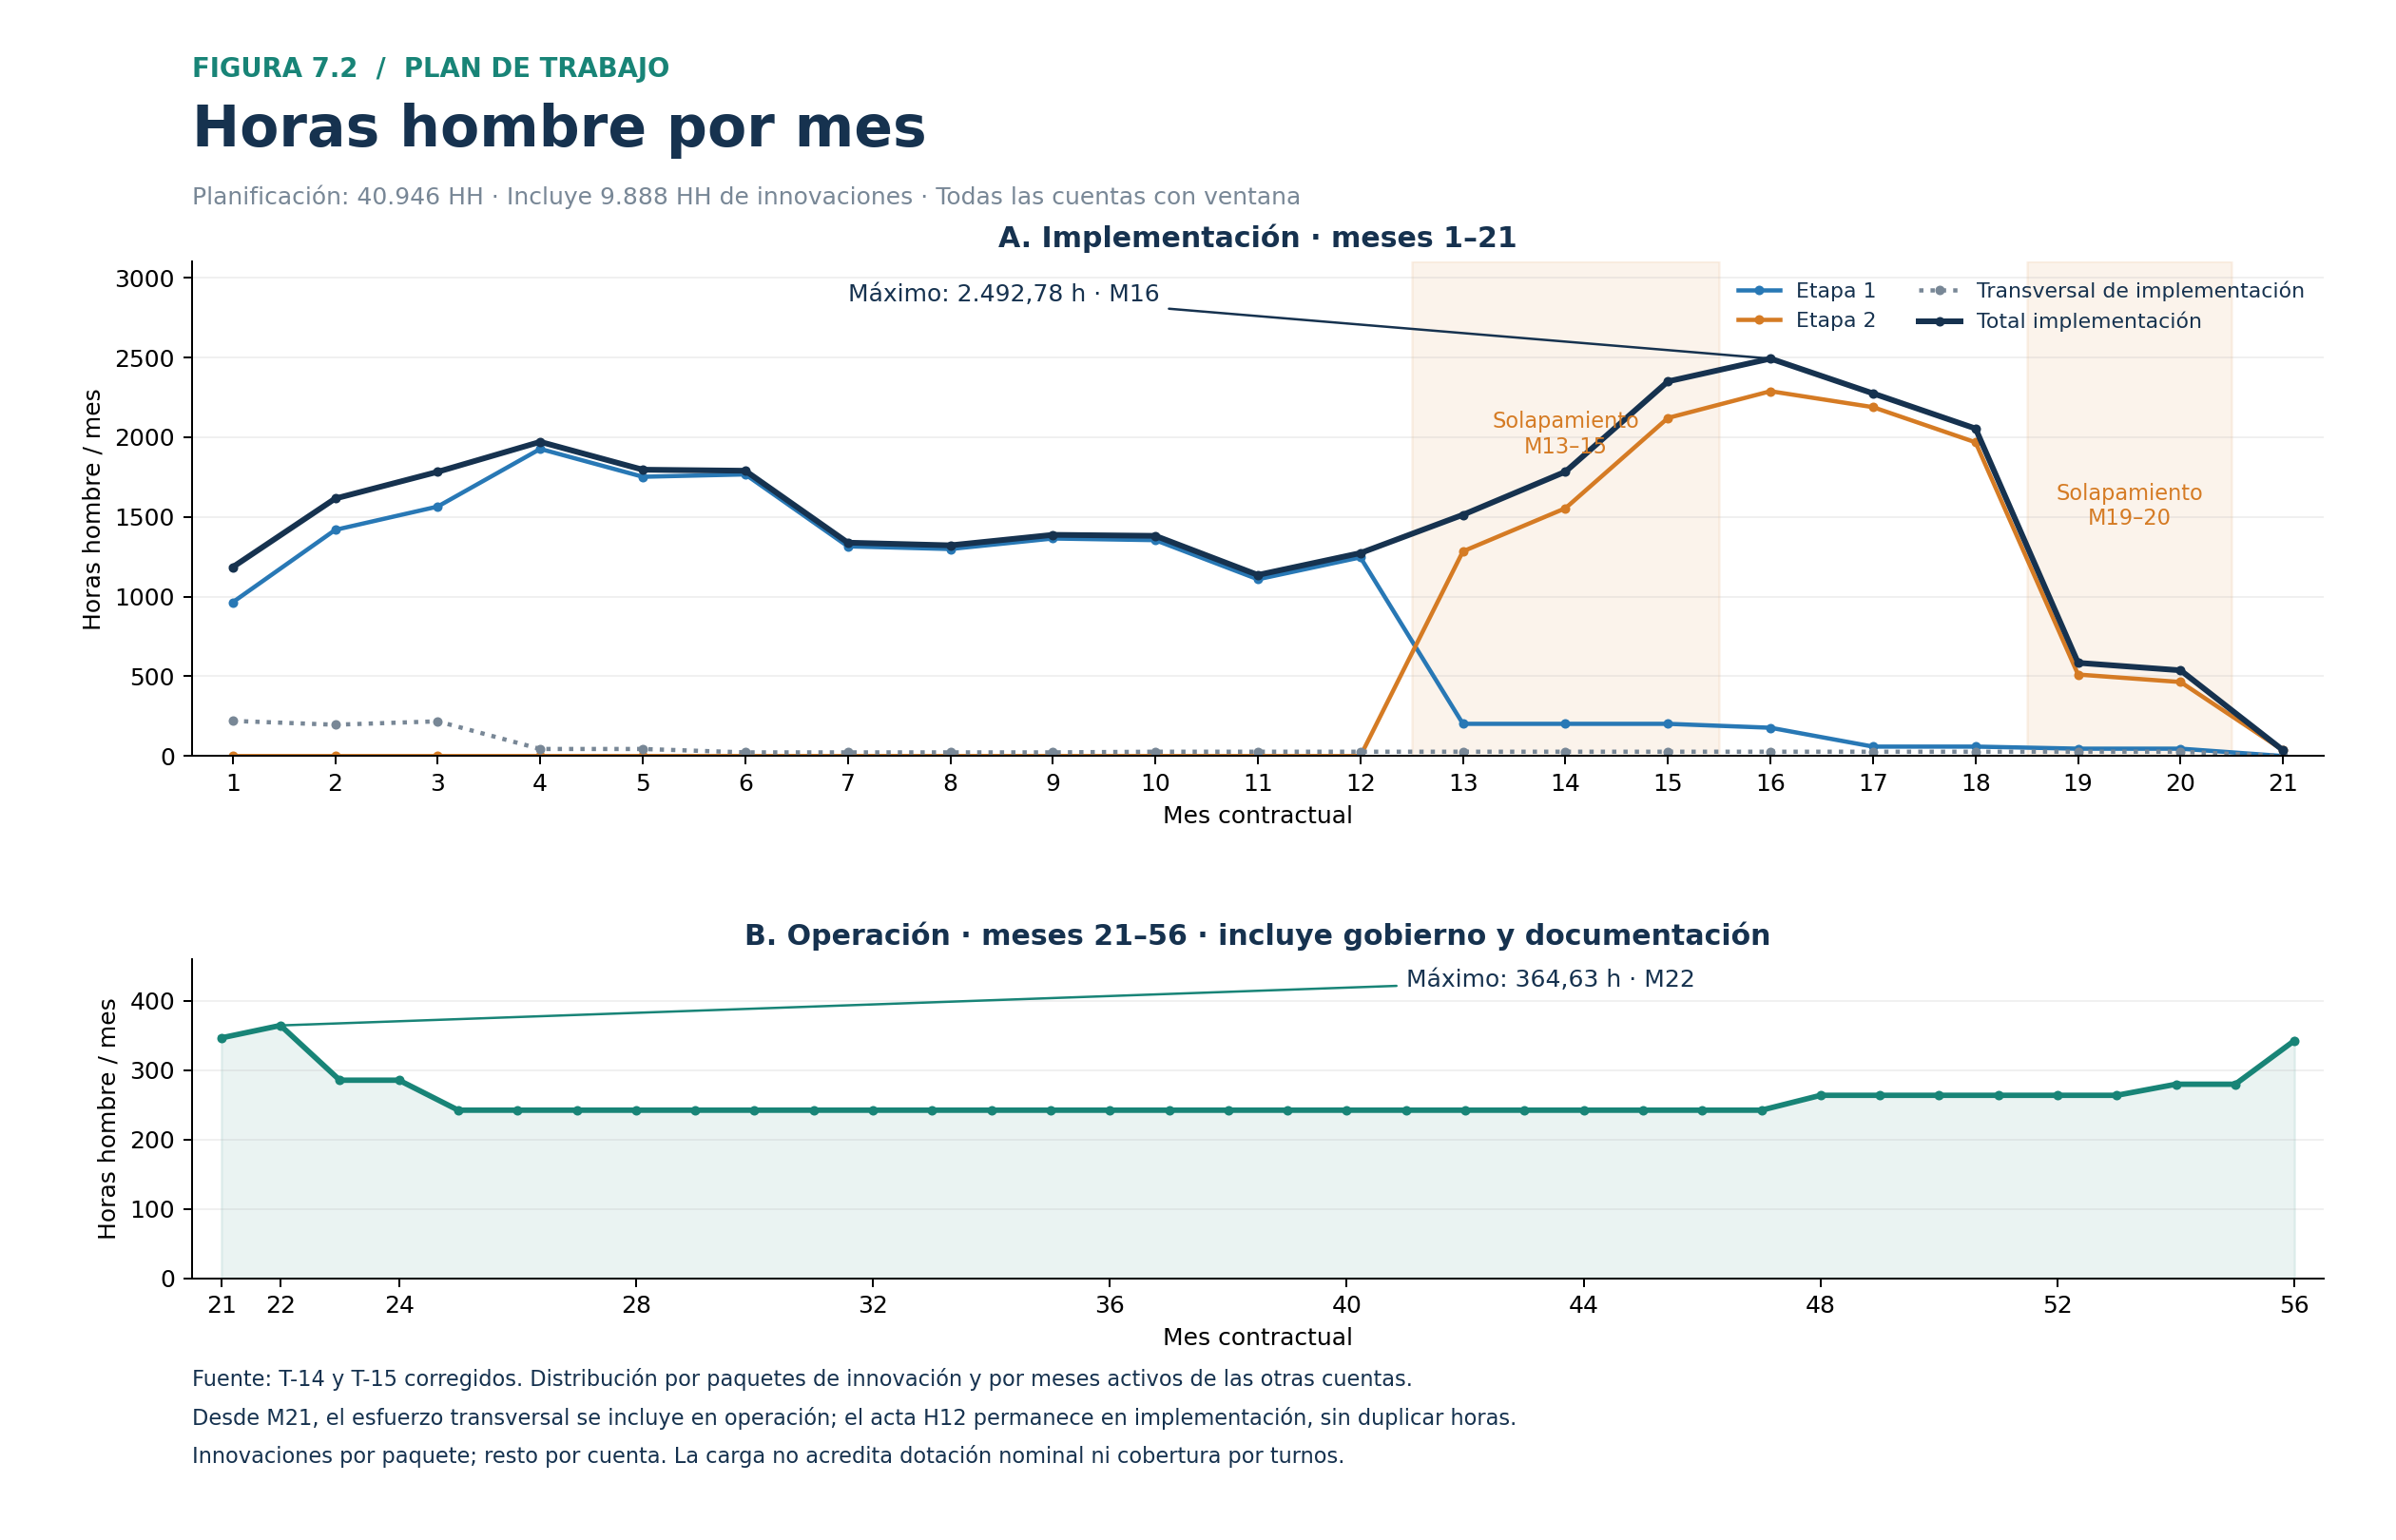
\includegraphics[width=\linewidth,height=\textheight,keepaspectratio]{figuras/sd07-figuras/sd07-73-curva-hh.png}
\raggedright\textbf{Fuente:} Elaboración propia a partir de T-14 y T-15.
\end{minipage}
\end{center}

La implementación alcanza su máximo de 2.492,78 HH en M16. La operación alcanza 364,63 HH en M22, después de distribuir el acompañamiento final entre M54 y M56. Las franjas M13--15 y M19--20 representan coexistencia de frentes. La curva incluye las 9.888 HH de innovaciones y su seguimiento; el total planificado alcanza 40.946 HH. La capacidad disponible por especialidad se contrasta con la demanda máxima de M16 antes de comprometer la ejecución.

\subsubsection{7.3.3.1 Margen de las innovaciones y del cierre}

Los siete paquetes de implementación de cada innovación tienen holgura total y margen restante de cero meses. No se puede desplazar íntegramente su programación conservando las duraciones y los hitos. Con entregas parciales, una extensión de duración no retrasa necesariamente el hito si esas entregas se mantienen. Por ejemplo, ampliar de dos a tres meses el paquete 1.10.3.2 mantiene H12; desplazar su inicio un mes desplaza H12 un mes y resulta incompatible con el contrato. El jefe de proyecto confirma estas entregas parciales con los equipos y proveedores antes de comprometer su ejecución.

El retiro de la plataforma tiene margen cero respecto del objetivo interno M22, condicionado al cierre de migración en M21. La transferencia de nueve meses tiene una holgura total de 27 meses desde su inicio más temprano; al programarla en M48--56 ese margen ya está consumido. El acta final presenta la misma situación. La entrega del código por liberación y su custodia continúan durante el contrato.

Los servicios continuos y los ensayos periódicos se controlan mediante su frecuencia, sus fechas comprometidas y sus niveles de servicio. No se les asigna una holgura de 36 meses. El anexo CPM contiene la red y las fechas tempranas, tardías y programadas.

\subsection{7.3.4 Carta Gantt y relación con los hitos del Anexo E-25}

La Figura 7.18 muestra las ventanas mensuales de las cuentas y sus entregas parciales. Una cuenta puede tener varios tramos activos y más de un hito. Las cinco cuentas de innovación comprenden construcción, aceptación y seguimiento; sus paquetes detallan la carga de cada tramo. El Formulario T-14 presenta el calendario por cuenta. Los colores del Gantt distinguen tipos de tramo; las figuras por etapa emplean sus propias leyendas de holgura.

\begin{center}
\begin{minipage}{\linewidth}
\centering
\ossFigCaption{Carta Gantt de los 56 meses, con los tramos por cuenta de control, las bandas de cada etapa y los hitos de aceptación.}\label{fig:7-18}
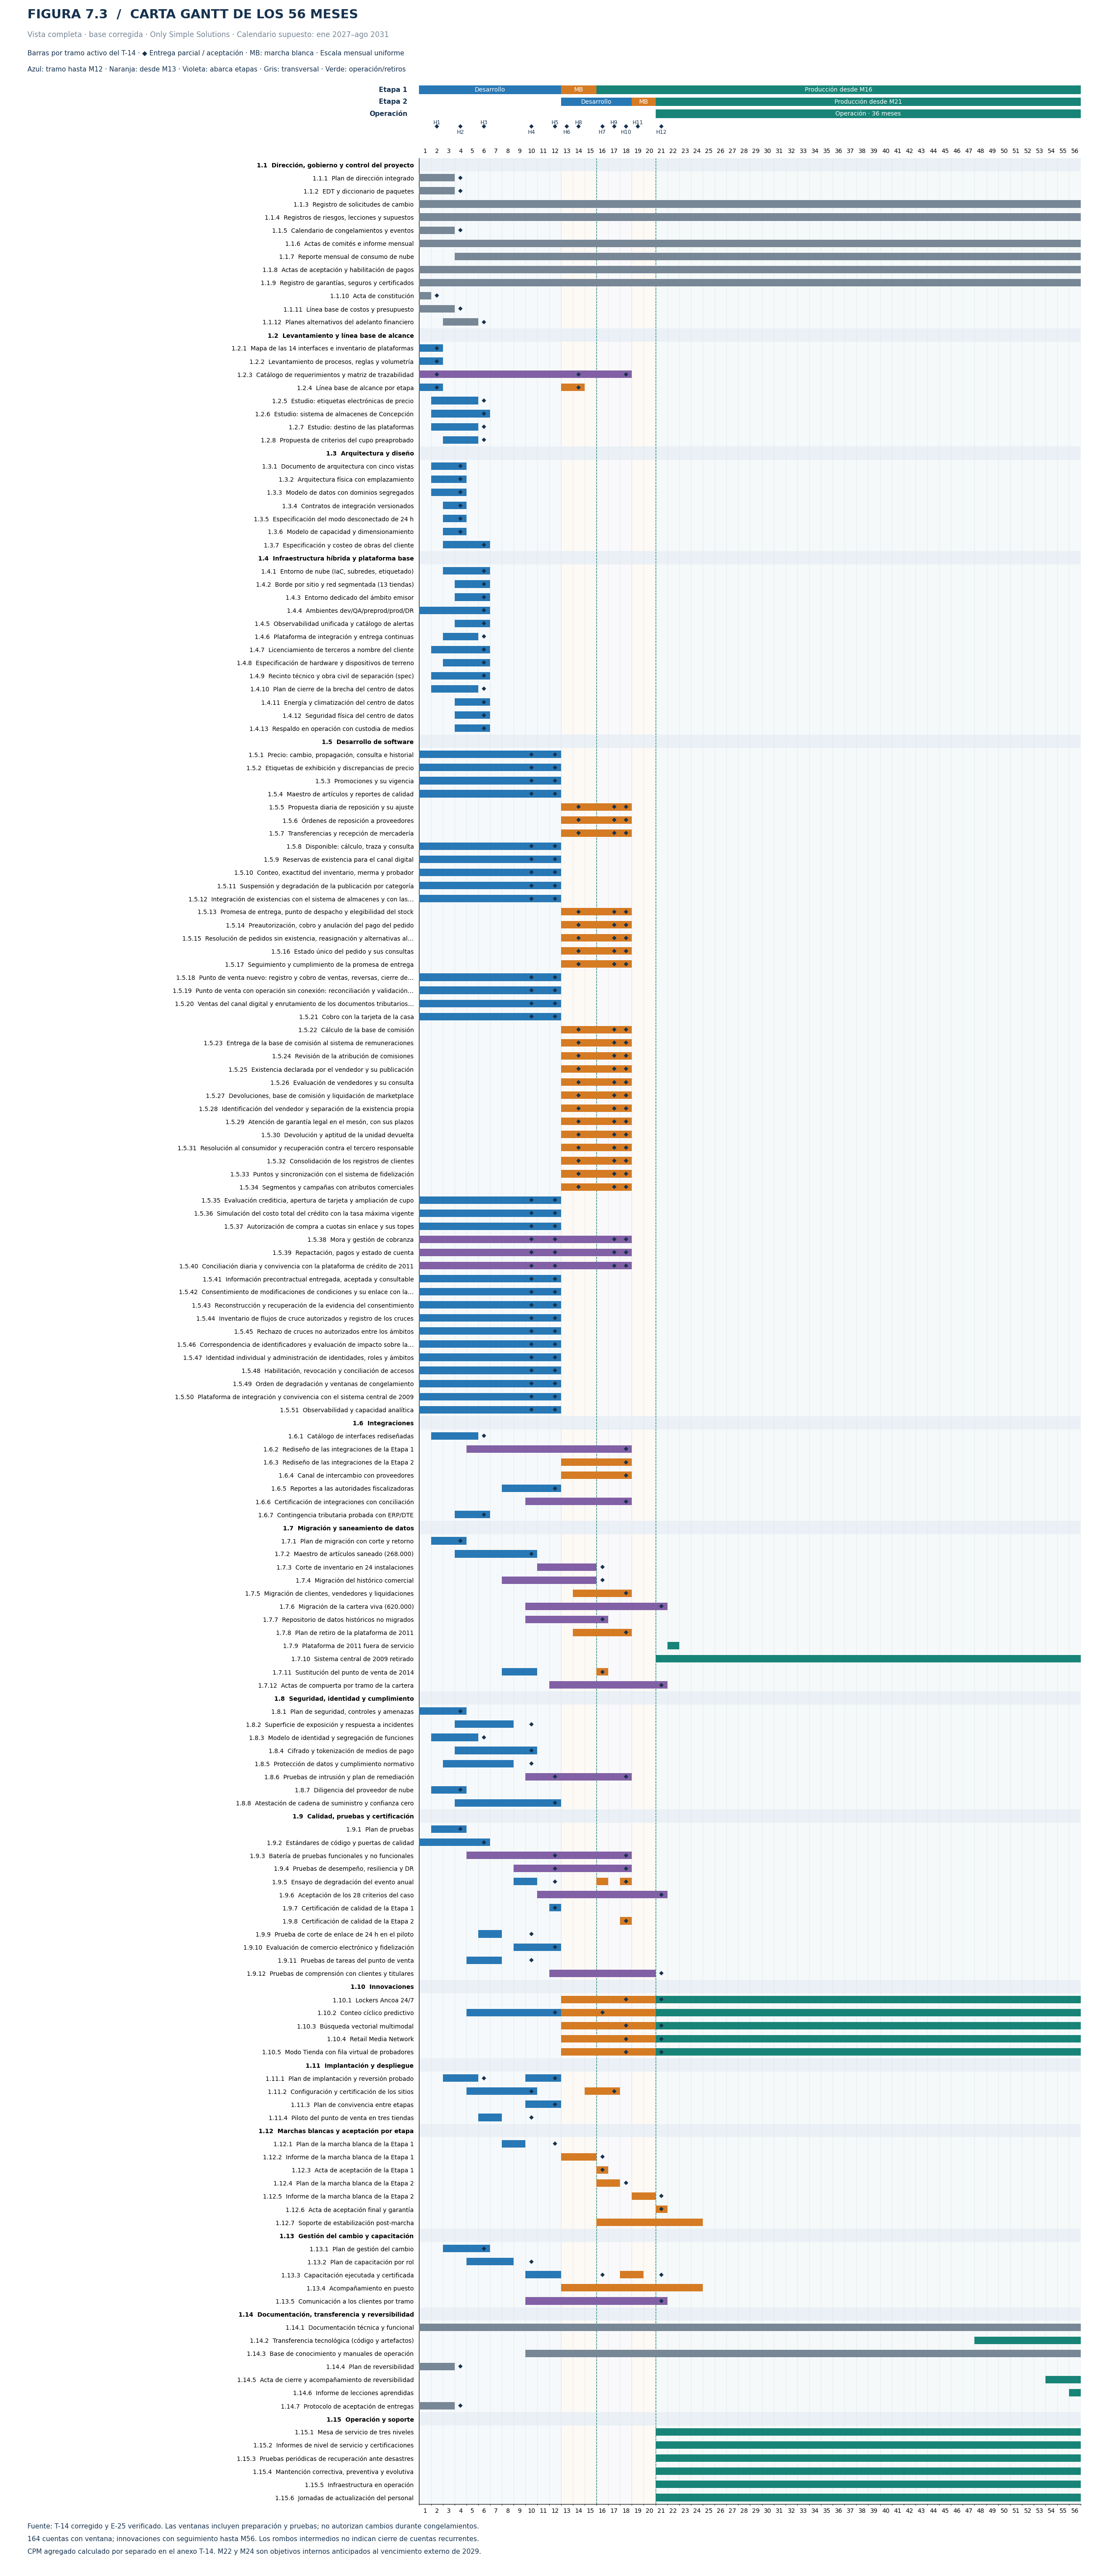
\includegraphics[width=\linewidth,height=0.78\textheight,keepaspectratio]{figuras/sd07-figuras/sd07-73-gantt.png}
\raggedleft\textbf{Fuente:} Elaboración propia a partir del T-14.
\end{minipage}
\end{center}

Las bandas superiores distinguen desarrollo, marcha blanca y producción por etapa. Las cuentas recurrentes mantienen trabajo después de su primera entrega; un rombo intermedio no indica que la cuenta completa haya terminado. H3 recibe ambientes en M6, el plan de convivencia precede a M13 y las pruebas de cada alcance se cierran antes de su marcha blanca. La vista general se complementa con los cronogramas de las etapas.

La Tabla 7.6 relaciona los hitos del Formulario E-25 con la evidencia principal de aceptación.

\begin{longtable}{p{0.09\linewidth}p{0.08\linewidth}p{0.71\linewidth}}
\caption{Hitos de aceptación.}\label{tab:7-6}\\
\toprule
\textbf{Hito} & \textbf{Mes} & \textbf{Evidencia principal} \\
\midrule
\endhead
\bottomrule
\multicolumn{3}{@{}l}{\rule{0pt}{3.2ex}\textbf{Fuente:} Elaboración propia a partir del Formulario E-25.} \\
\endlastfoot
H1 & 2 & Levantamiento, línea base y matriz aprobados \\
H2 & 4 & Arquitectura, seguridad y modelo de datos aprobados \\
H3 & 6 & Infraestructura y ambientes operativos con observabilidad \\
H4 & 10 & Software E1 para pruebas, QA superado y cobertura \\
H5 & 12 & Certificación E1 con pruebas aprobadas \\
H6 & 13 & Inicio de marcha blanca E1 y reversión activa \\
H8 & 14 & Línea base y diseño detallado E2 aprobados \\
H7 & 16 & Producción E1 y cierre conforme de marcha blanca \\
H9 & 17 & Software E2 para pruebas con QA superado \\
H10 & 18 & Certificación E2 y cierre del desarrollo \\
H11 & 19 & Inicio de marcha blanca E2 en convivencia \\
H12 & 21 & Producción E2 y aceptación final \\
\end{longtable}

H8 precede temporalmente a H7 aunque su identificador sea mayor. La aceptación exige el acta de la Contraparte Técnica; la entrega de un informe por sí sola no habilita el pago. La operación comprende 36 prestaciones mensuales M21--56, sin anticiparlas ni imputarlas a implementación.

\subsubsection{7.3.4.1 Etapa 1 — Preparación, desarrollo y primera puesta en producción}

La Etapa 1 prepara la base de la solución y entrega el alcance inicial que Ancoa utilizará en producción. Comprende el desarrollo M1--12, la marcha blanca M13--15 y la producción desde M16. La separación entre la actividad comercial y el emisor debe verificarse antes de construir una vista unificada de cliente (Multitiendas Ancoa S.A., 2026, Caso 09, cap. 13, núm. 13.3, condición 7, p. 30).

La secuencia comienza con el alcance y la arquitectura, seguidos de la integración de infraestructura y ambientes. Estos se habilitan progresivamente. El piloto técnico aislado de M6--7 aporta evidencia para preparar el despliegue; las ventas oficiales permanecen en los sistemas vigentes durante el ensayo. La construcción e integración final llega a H4 en M10 y las pruebas de cierre sustentan H5 en M12. En paralelo se preparan el plan de marcha blanca y la capacitación.

La Figura 7.19 presenta el CPM hasta H7, incluidos los siete paquetes de implementación del conteo predictivo. El rojo identifica holgura cero y el azul, margen disponible; el contorno discontinuo representa ese margen. El piloto conserva su ventana en el T-14, pero no integra la red CPM y no se le atribuye criticidad en esta vista.

\begin{center}
\begin{minipage}{\linewidth}
\centering
\ossFigCaption{Cronograma de la Etapa 1, cadena crítica y holguras hasta H7 en M16.}\label{fig:7-19}
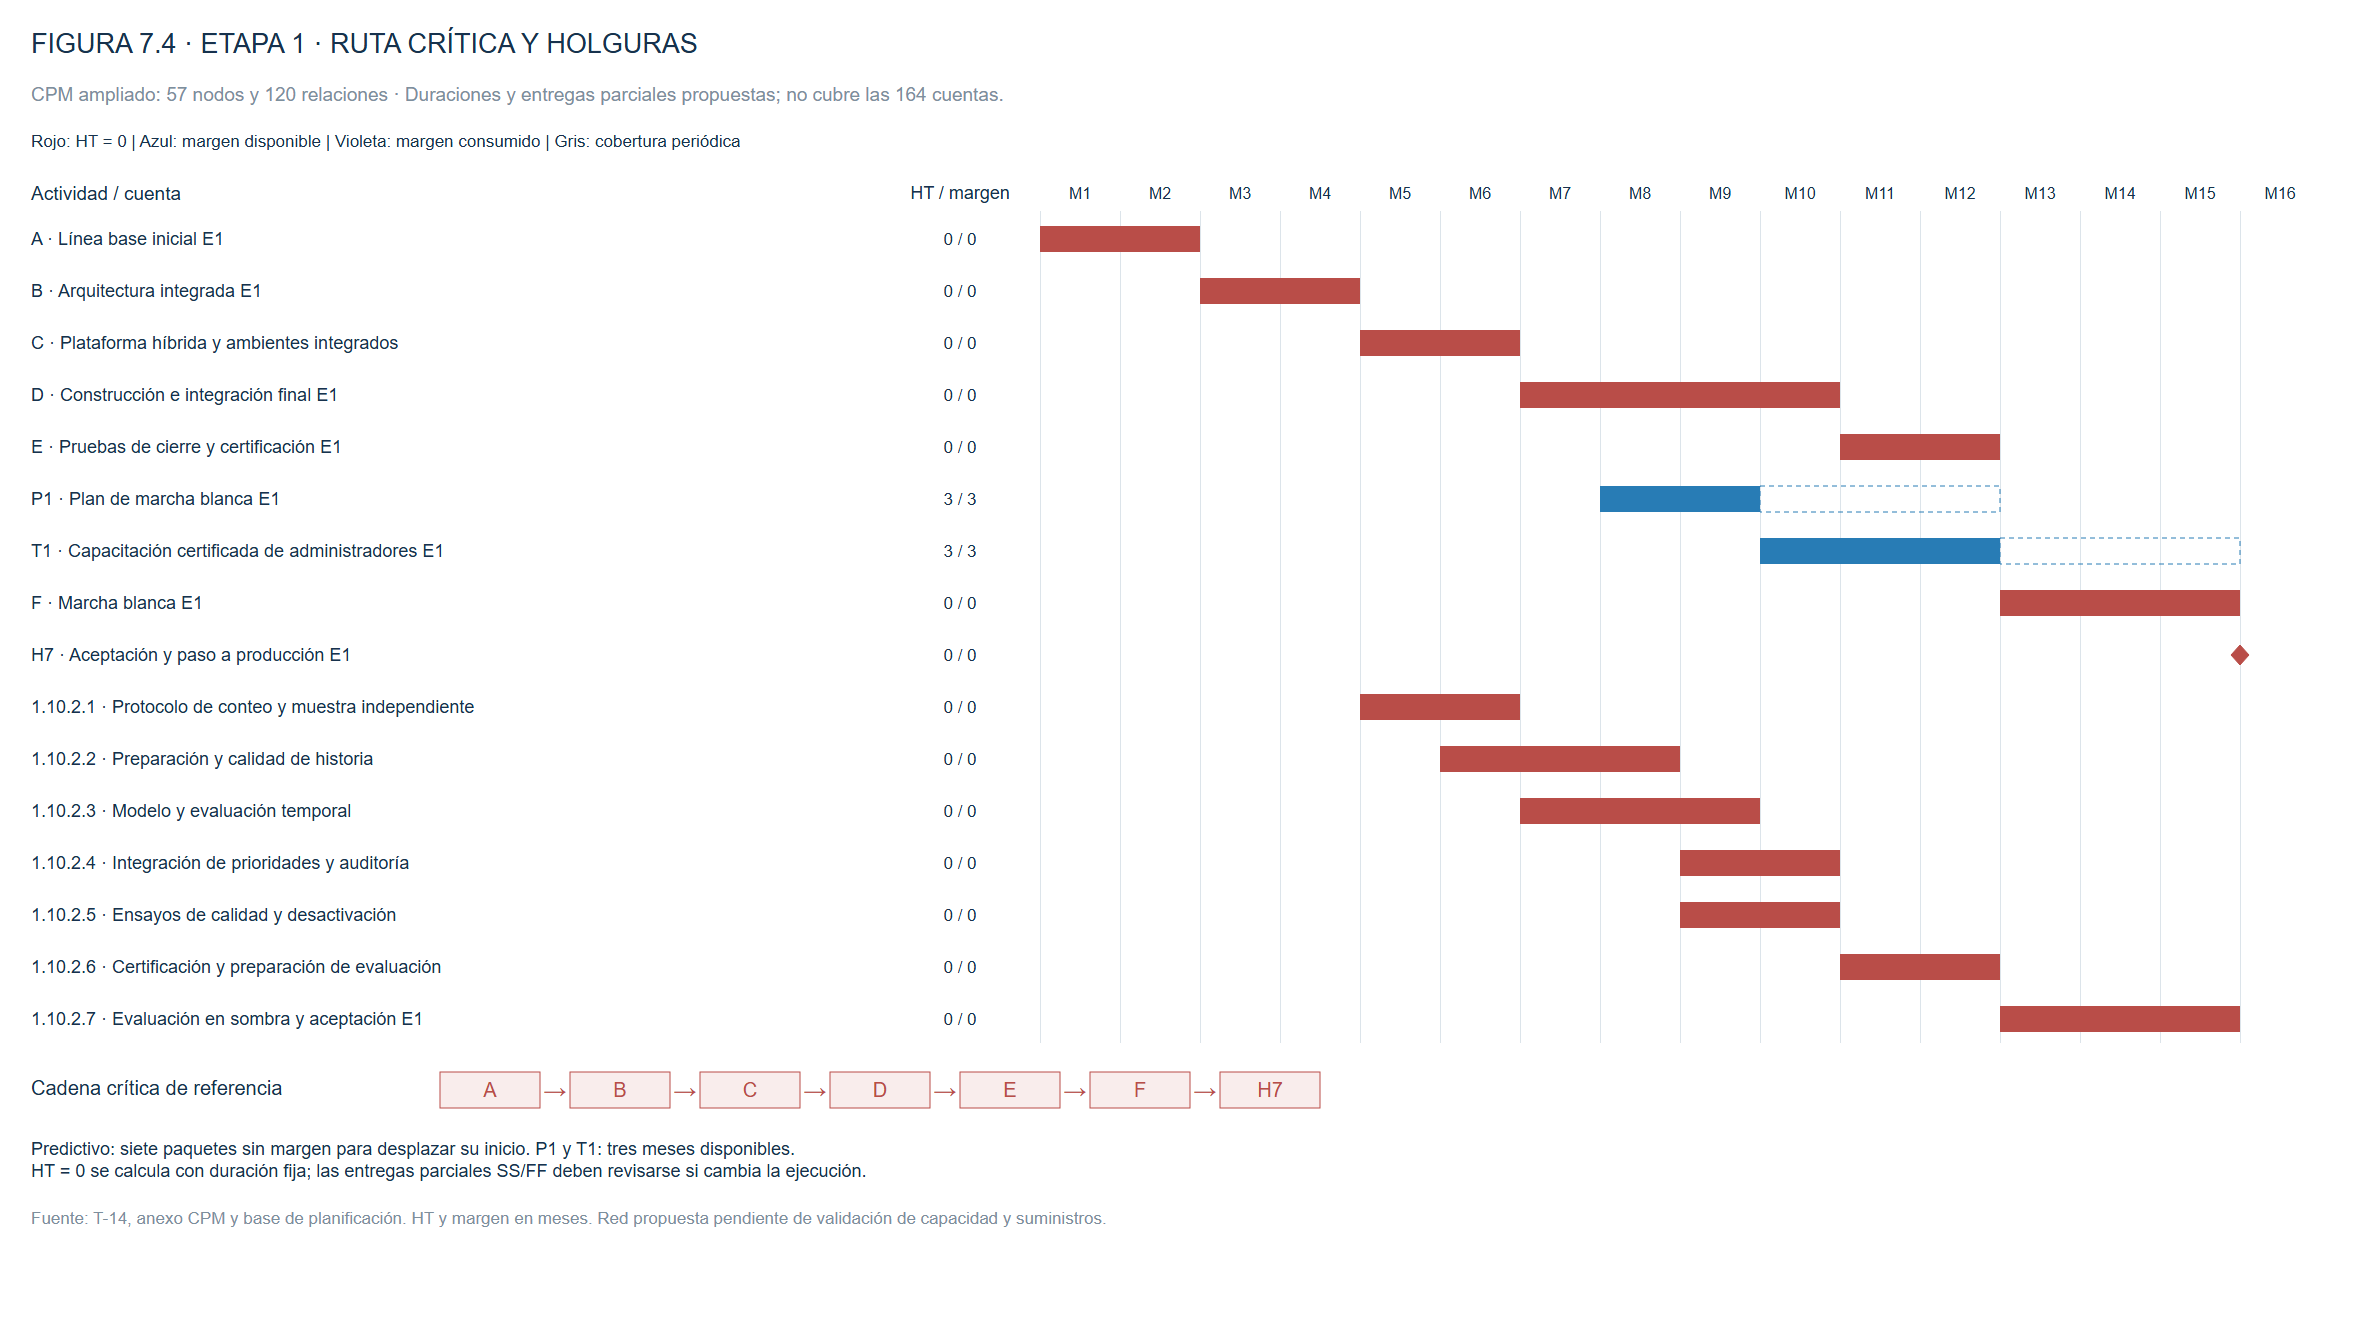
\includegraphics[width=\linewidth,height=\textheight,keepaspectratio]{figuras/sd07-figuras/sd07-73-etapa1.png}
\raggedright\textbf{Fuente:} Elaboración propia a partir del T-14 y su anexo CPM.
\end{minipage}
\end{center}

La cadena A--B--C--D--E--F--H7 tiene holgura cero. El plan P1 y la certificación de administradores T1 conservan tres meses cada uno. Estos márgenes no se trasladan automáticamente a las cuentas del T-14. La habilitación de usuarios debe estar resuelta antes de su incorporación a la operación supervisada. Entre M13 y M15 también comienza E2, por lo que ambos equipos coordinan cambios y ambientes compartidos. La aceptación E1 requiere demostrar las condiciones de cierre desarrolladas en el T-18.

\subsubsection{7.3.4.2 Etapa 2 — Ampliación de la solución y convivencia con la Etapa 1}

La Etapa 2 incorpora el alcance adicional de la segunda entrega. Su desarrollo ocupa M13--18, la marcha blanca M19--20 y el paso a producción M21. Al comenzar, E1 sigue en marcha blanca; desde M16 debe convivir con ella en producción. Los trabajos de ampliación preservan los servicios aceptados y la coherencia de los datos.

La línea base y el diseño detallado se preparan en M13--14 y se aceptan en H8. La construcción e integración se concentran en M15--17, con entrega para pruebas en H9. La certificación M18, asociada a H10, precede a H11. El plan de marcha blanca se prepara en M16--17. La certificación de administradores se programa en M18--19, sin desplazar la capacitación necesaria para participar desde el inicio.

La Figura 7.20 muestra la cadena crítica y los 28 paquetes de las otras cuatro innovaciones. Conserva los meses contractuales M13--21 para comparar sus fechas con el Gantt general. La certificación E de la primera etapa es un antecedente externo a esta ventana.

\begin{center}
\begin{minipage}{\linewidth}
\centering
\ossFigCaption{Cronograma de la Etapa 2, cadena crítica y holguras hasta H12 en M21.}\label{fig:7-20}
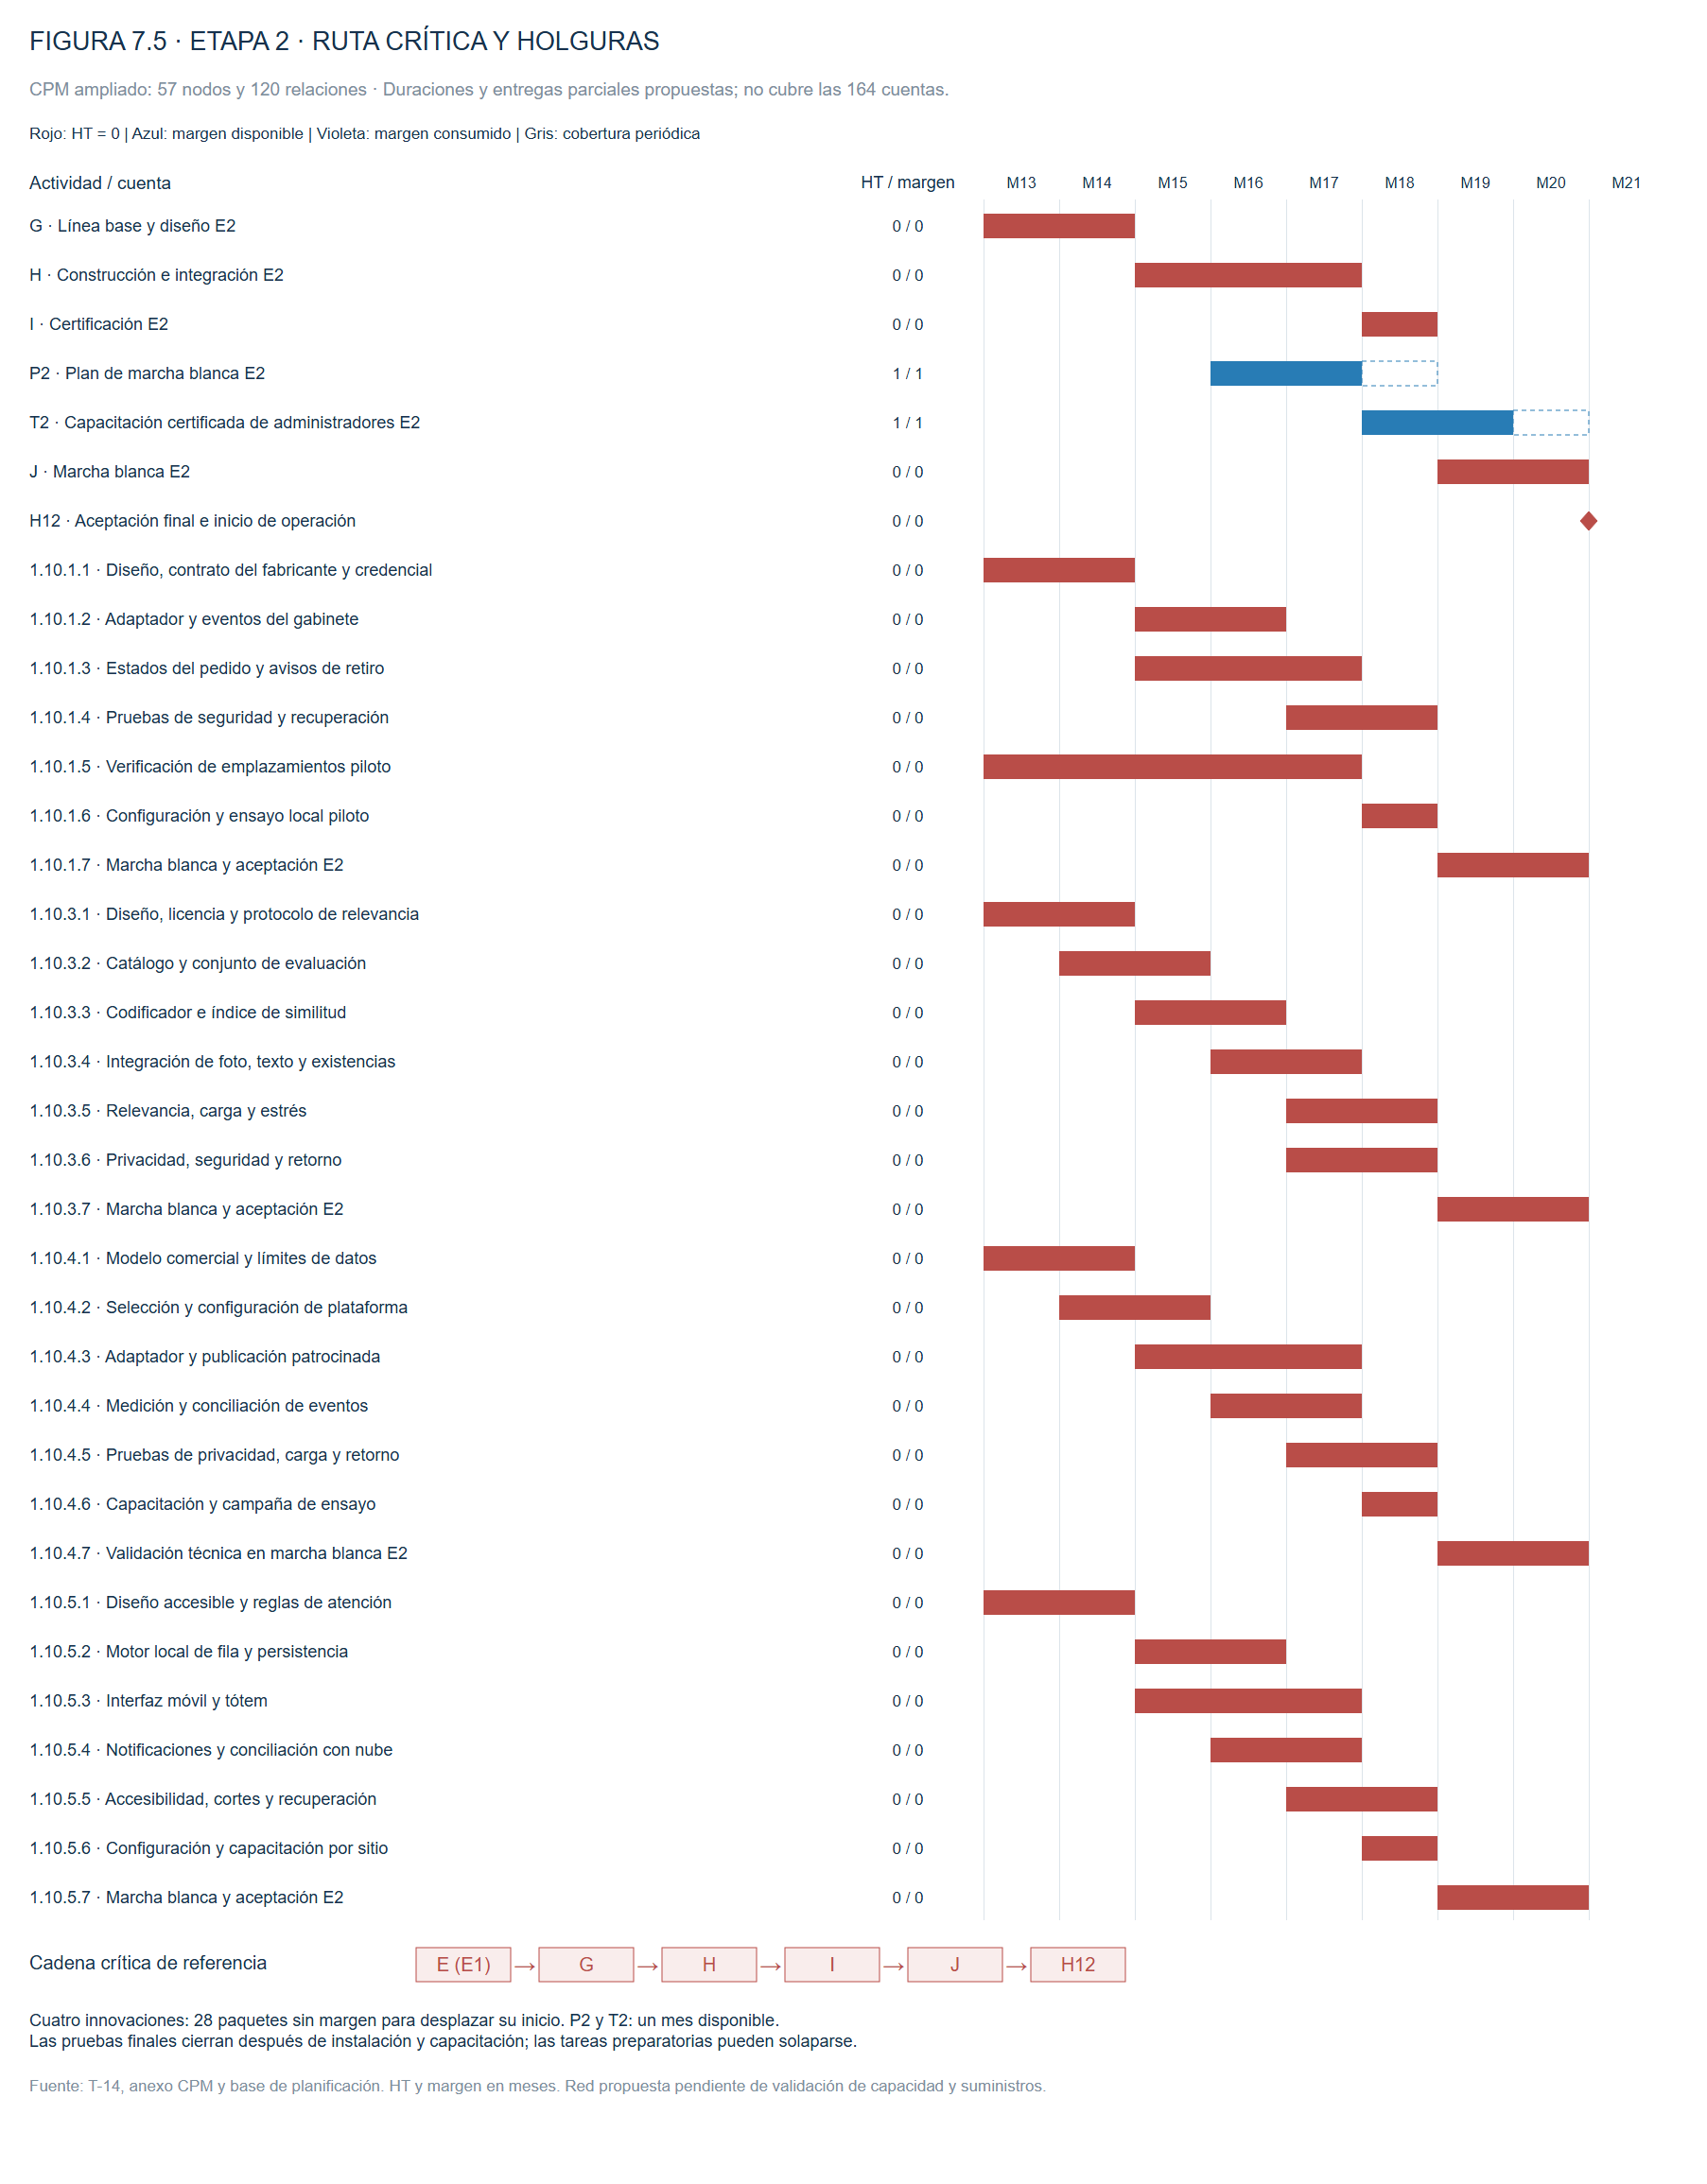
\includegraphics[width=\linewidth,height=\textheight,keepaspectratio]{figuras/sd07-figuras/sd07-73-etapa2.png}
\raggedright\textbf{Fuente:} Elaboración propia a partir del T-14, su anexo CPM y los hitos del Formulario E-25.
\end{minipage}
\end{center}

La secuencia E--G--H--I--J--H12 conserva holgura cero. Su tramo previo A--B--C--D--E aparece en la Figura 7.19. P2 y T2 tienen un mes de margen cada uno. H12 depende además de H7 y requiere los resultados de marcha blanca, conciliación y capacitación. En M21 coinciden la producción E2 y el inicio de operación, sin duplicar el esfuerzo entre ambas prestaciones.

\subsubsection{7.3.4.3 Operación — Continuidad del servicio y cierre contractual}

La operación comprende los 36 meses M21--56. Sostiene el servicio aceptado, atiende incidentes y realiza el mantenimiento comprometido. Incluye mesa de servicio, administración de infraestructura e informes de cumplimiento. Los ensayos de recuperación y la actualización del personal se ejecutan con sus frecuencias previstas.

La estabilización continúa hasta M24 y el retiro de la plataforma de crédito se programa en M22 como objetivo interno anticipado. La documentación se mantiene vigente durante el servicio. La transferencia tecnológica M48--56 prepara el traspaso final, cuyo cierre se registra en M56.

La Figura 7.21 distingue la operación contractual, el retiro, la transferencia y el cierre. El rojo indica holgura cero; el violeta, holgura ya consumida por las fechas programadas. Las barras grises representan obligaciones periódicas que no tienen una holgura única. El acompañamiento final se programa en M54--56, con inicio efectivo al menos 90 días antes del término.

\begin{center}
\begin{minipage}{\linewidth}
\centering
\ossFigCaption{Cronograma de operación, plazo crítico agregado y ventanas de servicio, M21--56.}\label{fig:7-21}
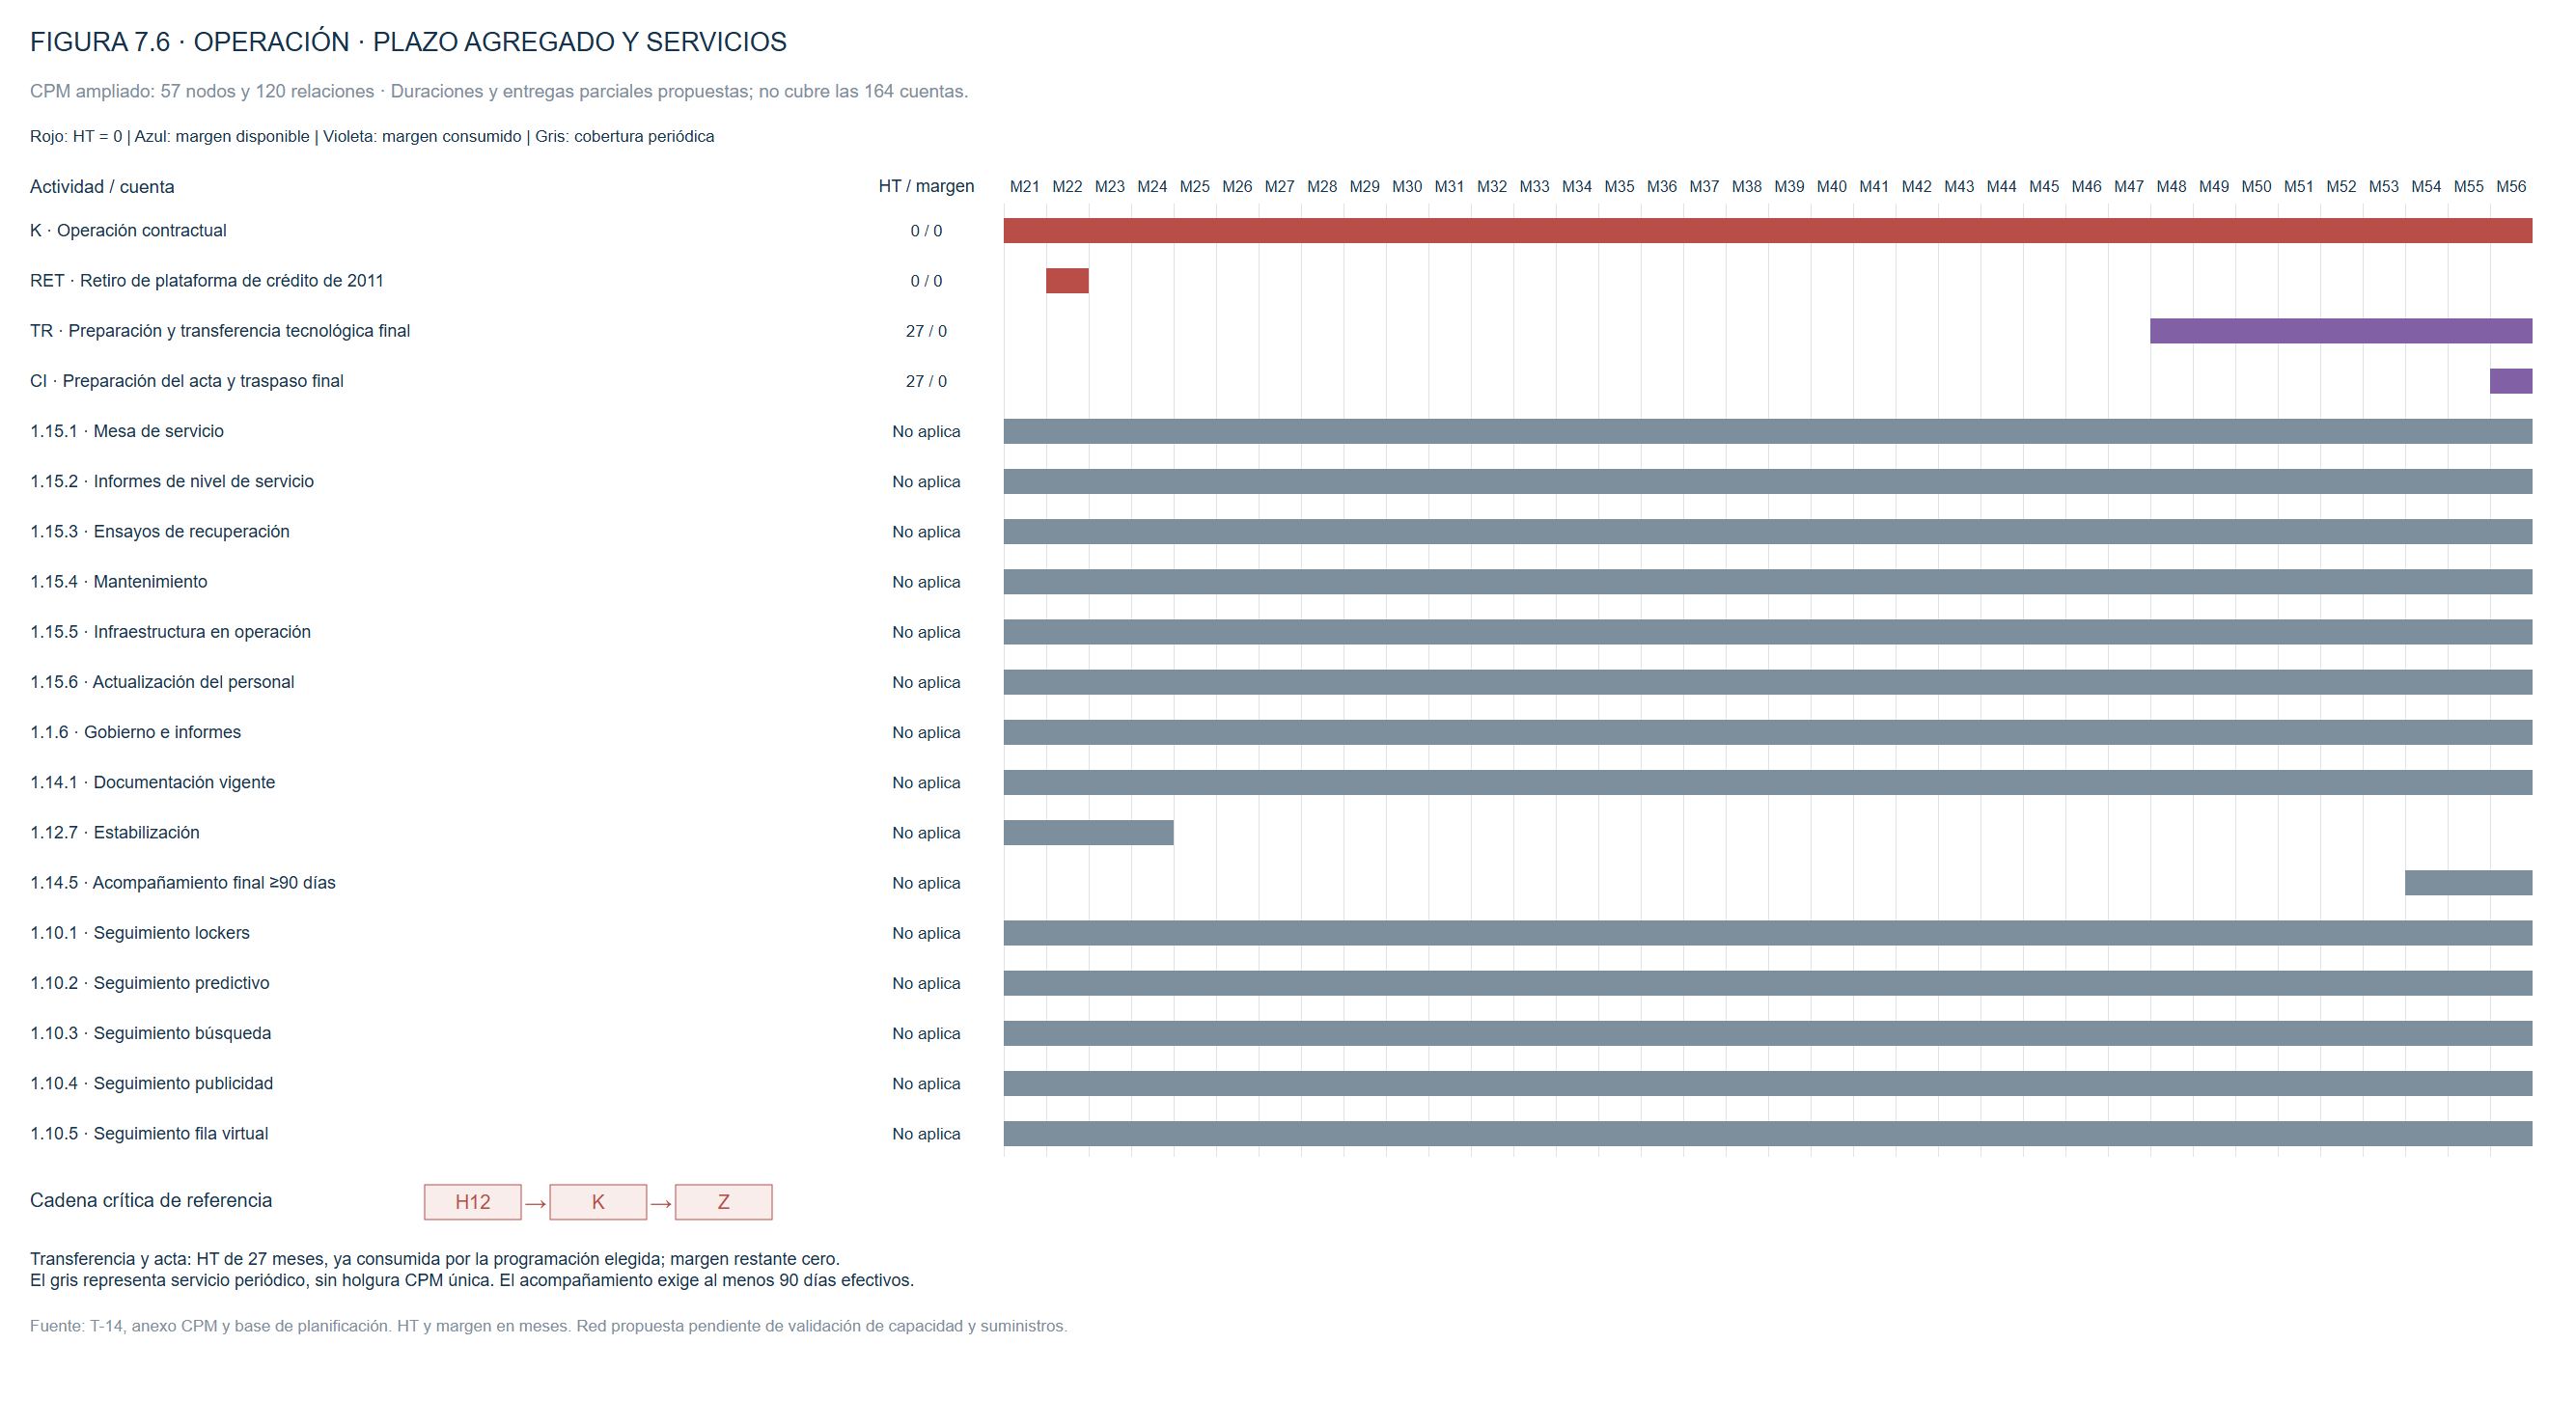
\includegraphics[width=\linewidth,height=\textheight,keepaspectratio]{figuras/sd07-figuras/sd07-73-operacion.png}
\raggedright\textbf{Fuente:} Elaboración propia a partir del T-14 y de la planificación mensual del T-15.
\end{minipage}
\end{center}

Las barras largas representan obligaciones vigentes durante la operación. Las pruebas de recuperación comprenden al menos dos ejecuciones al año y la actualización del personal, al menos dos jornadas anuales (RT-22.06). Los informes mensuales permiten comprobar los niveles de servicio. La dotación por rol y la cobertura de atención deben contrastarse con los capítulos de equipo y operación para demostrar que los recursos permiten cumplir esas obligaciones.

Los 35 paquetes de implementación de las innovaciones tienen holgura cero bajo las duraciones y dependencias previstas. Su seguimiento durante la operación comprende cinco paquetes de actividades periódicas.

\subsection{7.3.5 Plan de implantación}

El T-18 desarrolla la puesta en servicio por oleadas, las pruebas y la reversión. La estrategia responde a la convivencia previa, la continuidad de venta y cobro y el despliegue por tienda, proceso o categoría exigidos para Ancoa (Multitiendas Ancoa S.A., 2026, Caso 09, cap. 13, núm. 13.3, condiciones 1--4, pp. 29--30). Como decisión de planificación, en M6--7 se propone un piloto técnico del punto de venta en tres tiendas, en preproducción aislada y fuera de congelamientos. El ensayo propuesto de corte de enlace de 24 horas afecta al entorno de prueba, mientras los sistemas vigentes sostienen venta y cobro. La convivencia con datos y usuarios reales se acredita durante M13--15 y el cambio de registro oficial por tienda ocurre desde M16.

La cuenta 1.7.11 separa la preparación M8--10 del cambio productivo M16. Las banderas de función controlan la liberación, sin autorizar intervenciones durante congelamientos. El despliegue mantiene la separación Retail--Emisor, la conciliación por dominio y el retorno probado por tramo de cartera. La migración de los 620.000 clientes con saldo requiere convivencia real, conciliación diaria y un plan de comunicación, sin una fecha única de corte sin respaldo (Multitiendas Ancoa S.A., 2026, Caso 09, cap. 13, núm. 13.3, condiciones 5 y 7, p. 30).

Antes de cada aceptación se presentan pruebas funcionales, de seguridad, resiliencia y recuperación, de carga a 1,5 veces el máximo declarado y de estrés hasta el punto de quiebre. Los indicadores y evidencias se trazan a los 28 resultados de aceptación del caso (Multitiendas Ancoa S.A., 2026, Caso 09, cap. 18, pp. 44--45). Además, se comprueba el cumplimiento de los umbrales técnicos aplicables. El T-18 distingue los umbrales obligatorios de las mejoras que requieren una línea base acordada; una media corporativa no constituye por sí sola un volumen de aceptación aprobado por sitio.

Cada reversión se ensaya antes de exponer el alcance. El procedimiento conserva las transacciones efectuadas durante la convivencia y las concilia con la versión restaurada. Recuperar una copia antigua sin tratar las operaciones posteriores no permite acreditar la integridad de la cartera.

\subsubsection{7.3.5.1 Liberación por componente y decisión de retorno}

Conforme a 6.2.5, los servicios de nube utilizan despliegue azul-verde. La nueva versión se prepara en un entorno equivalente y el tráfico cambia hacia ella después de superar las pruebas y la autorización de liberación. La versión anterior permanece disponible durante la observación. En tiendas, una primera tienda recibe la liberación como canario y las siguientes avanzan por oleadas una vez verificados los indicadores. Este canario productivo es distinto del piloto técnico aislado de M6--7.

El dominio financiero mantiene su despliegue segregado en el entorno local. La migración avanza por tramos de cartera conciliados, con control del Líder de Datos y del Encargado de Seguridad. La reversión de la aplicación se automatiza solo cuando se ha probado su compatibilidad con los datos. Una diferencia de saldos o una vulneración de la frontera de datos detiene el avance y activa la contención y conciliación del T-18.

Antes de cada oleada, Operación y Calidad configuran los umbrales de disponibilidad, respuesta y errores del servicio y el período de observación aprobado. El proceso de despliegue ejecuta el retorno automático si se incumple una condición configurada y el ensayo demostró que el retorno conserva las transacciones. Si volver atrás exige transformar o restaurar datos, se bloquea la expansión y Operación coordina el retorno asistido con Datos. Ninguna oleada continúa mientras exista una condición bloqueante.

\subsection{7.3.6 Marcha blanca y criterios de cierre}

Las cuentas 1.12.1 y 1.12.4 preparan los planes de marcha blanca E1 y E2; las cuentas 1.12.2 y 1.12.5 registran sus resultados en M13--15 y M19--20. El cierre exige conjuntamente las seis condiciones de aceptación desarrolladas en el T-18.

Deben estar cerrados los incidentes críticos y altos atribuibles a la solución. Durante al menos las cuatro últimas semanas debe alcanzarse el volumen real comprometido y sostenerse la disponibilidad y los tiempos de respuesta. La conciliación no debe presentar diferencias no explicadas, el personal debe estar capacitado y certificado conforme al plan aprobado y la Contraparte Técnica debe firmar el acta correspondiente.

Si alguna condición falla, la marcha blanca se extiende a costo del adjudicatario, sin desplazar las fechas contractuales siguientes y con las consecuencias contractuales aplicables. El plan de recuperación identifica trabajo, responsables y evidencia de cierre. La fecha programada no equivale a una aceptación automática.

La trazabilidad utiliza el código de cuenta del T-14 para relacionar esfuerzo del T-15, ventana del Gantt, hito y evidencia del T-18. Los números de tabla y figura son referencias editoriales distintas de esos códigos.


\section*{Referencias}
\addcontentsline{toc}{section}{Referencias}



\section*{Declaración de uso de IA}
\addcontentsline{toc}{section}{Declaración de uso de IA}



\ossFinalPage

\end{document}
